%! suppress = Makeatletter
%! suppress = Makeatletter
\documentclass[11pt]{report}

\usepackage[T1]{fontenc}
\usepackage[utf8]{inputenc}
\usepackage{graphicx}
\usepackage{amsmath,amssymb,amsfonts}
\usepackage{polski}
\usepackage[raggedright]{titlesec}
\usepackage{indentfirst}
\usepackage{listings}
\usepackage{hyperref}
\usepackage[backend=biber, bibencoding=utf8, style=ieee, dashed=false, isbn=false, doi=false, sorting=anyvt]{biblatex}

\addbibresource{library.bib}

\pagestyle{headings}

\renewcommand{\chaptername}{Rozdział}
\renewcommand{\contentsname}{Spis treści}
\renewcommand{\figurename}{Rys.}
\renewcommand{\tablename}{Tab.}
\renewcommand{\listfigurename}{Spis rysunków}
\renewcommand{\listtablename}{Spis tabel}
\renewcommand{\bibname}{Bibliografia}

\makeatletter
\renewcommand{\l@section}{\@dottedtocline{1}{1.5em}{2.6em}}
\renewcommand{\l@subsection}{\@dottedtocline{2}{4.0em}{3.6em}}
\renewcommand{\l@subsubsection}{\@dottedtocline{3}{7.4em}{4.5em}}
\makeatother


\begin{document}

    \begin{titlepage}
        \centering
        
\includegraphics[width=1 \textwidth]{fig/AGH.jpg}
        \center{\scshape WYDZIAŁ INFORMATYKI, ELEKTRONIKI\\ I TELEKOMUNIKACJI\\
        Kierunek Informatyka}
        \vspace{0.03\textheight}
        \center{\scshape Michał Patyk}
        \bigskip
        \center{\LARGE\bfseries Analiza danych i wzorców dotyczących wydarzeń politycznych na podstawie informacji zgromadzonych w projekcie GDELT}
        \center{(pracownia problemowa)}
        \vspace{0.2\textheight}
        \par
        \rightline{Opiekun: dr hab. inż. Koźlak Jarosław}

        \vspace{0.1\textheight}
        \center{Kraków 2020}
    \end{titlepage}

    \tableofcontents


    \chapter{Wstęp}
    //Wydarzenia są opisywane przez zaangażowanych aktorów (którymi mogą być państwa lub specyficzne organizacje) oraz lokalizacje i kategorie definiujące charakter wydarzeń (np. różne rodzaje negocjacji , deklaracji politycznych, zamieszki, konflikty zbrojne, itp.), co jest specyfikowane przez zestawy szczegółowych atrybutów.

    //Postawić problem
    //dlaczego chemy realizować
    //na podstawie analiz chcemy lepiej zrozumieć specyfikę krajów
    //chęć automatycznej reakcji na to że cos sie dzieje
    //informacja o zdarzeniach nietypowych
    //jak społeczności reagują
    //patrz dyplom KKI


    \section{Cele pracy}
    Celem niniejszej pracy jest analiza wydarzeń politycznych oraz poszukiwanie występujących w nich wzorców w oparciu o dane projektu GDELT.


    \chapter{Przegląd dziedziny}
    W tym rozdziale opisany został zbiór danych GDELT, schemat kodwania CAMEO oraz przeprowadzony został przegląd istniejących analiz zbioru.


    \section{GDELT}
    GDELT - Global Database of Events, Language, and Tone - to największa, najbardziej wszechstronna i otwarta baza danych jaka powstała.
    Wczesne poszukiwania prowadzące do stworzenia GDELT zostały opisane przez Philipa Schrodta w dokumencie~\cite{Schrodt2010} w styczniu 2010 r.
    Zbiór danych jest dostępny na stronie Projektu ~\cite{gdelt} oraz na platformie Google Cloud gdzie można z niego korzystać przez Google BigQuery~\cite{BigQuery2014}.
    GDELT używa kodowania obserwacji konfliktów i mediacji (CAMEO)~\cite{GDELTDocumentation} do rejestrowania zdarzeń.
    W zbiorze znajdują się dane od 1979 roku.
    Kolejne porcje zdarzeń i ich klasyfikacja generowane sa na bieżąco każdego dnia.


    \section{CAMEO}
    CAMEO - Conflict and Mediation Event Observations - jest schematem kodowania zdarzeń.
    Został stworzony w Katedrze Nauk Politycznych Pennsylvania State University.
    Jego początki sięgają roku 2000.
    Został zaprojektowany z myślą o automatycznym kodowaniu i szczegółowym kodowaniu aktorów.

    \subsection{Zdarzenia}
    Kody zdarzeń są ujednolicone pod względem kolejności numerycznej głównych kategorii.
    Kategorie są uszeregowane rosnąco względem kooperacji od 01 do 09 oraz względem konfliktu od 10 do 20.

    \subsection{Aktorzy}
    Kody aktorów składają sie z trzech znaków.
    Elementy kodu są podzielone na szerokie kategorie, takie jak podmioty państwowe, role, regiony i grupy etniczne aktorów.


    \section{Przegląd istniejących analiz} \label{ch:przeglad}
    // artykuły analizujące, kto cytował, jakie analizy


    \chapter{Koncepcja}
    // jaki system chcemy stworzyć
    // wektory, algorytmy klastrowania

    W tym rozdziale zostały opisane\ldots


    \section{Założenia i wymagania}
    W analizie wykorzystany zostanie głównie zbiór danych GDELT 2.0 od początku 2015 roku do kwietnia 2020.


    \section{Efekt końcowy}
    Planowanym efektem końcowym pracy będzie\ldots


    \chapter{Realizacja}


    \section{Wykorzystane narzędzia}

    \begin{enumerate}
        \item[•] język programowania Python~\cite{python}
        \item[•] biblioteka Pandas~\cite{pandas}
        \item[•] biblioteka GeoPandas~\cite{geopandas}
        \item[•] biblioteka Scikit-Learn~\cite{scikit}
        \item[•] środowisko programistyczne PyCharm~\cite{pycharm}
        \item[•] internetowe interaktywne środowisko obliczeniowe Notebook Jupyter~\cite{jupyter}
        \item[•] hurtownia danych Google BigQuery~\cite{bigquery}
    \end{enumerate}

    // dyskusja co można by wykorzystac zamiast tych narzędzi np dane lokalne zamiast bigQuery

    Przy tworzniu projektu wykorzystany został język programowania Python.
    Jest to język wysokiego poziomu ogólnego przeznaczenia.
    Wraz z biblioteka Pandas jest często stosowany w zagadnieniach analizy danych oraz data miningu.
    Głównym narzędziem używanym do programowania było zintegrowane środowisko programistyczne PyCharm firmy JetBrains.
    Pozwala ono na wygodną edycję i analizę kodu źródłowego.
    Internetowe interaktywne środowisko obliczeniowe Notebook Jupyter pozwoliło na tworzenie dokumentów zawierających kod wraz z wizualizacjami.
    Wykorzystanie hurtowni danych Google BigQuery pozwoliło na szybką, skalowalną analizę dużego zbioru danych jakim jest GDELT.
    BigQuery jest oprogramowaniem bezserwerowym, które obsługuje zapytania w języku ANSI SQL.
    Podział krajów na klastry został wykonany przy użyciu Scikit-Learn.
    Do wizualizacji klastrów na mapie wykorzystano bibliotekę GeoPandas.


    \section{Wstępna analiza danych}
    W tej części pracy przeprowadzona zostanie wstępna analiza zagregowanych danych. W pierwszej kolejności przeanalizowane zostaną dane dotyczące Polski, co pozwoli na łatwiejsze wychwycenie związków między zarejestrowanymi wydarzeniami, a sytuacją w kraju.
    W dalszej kolejności przeprowadzona zostania analiza zbiorcza dla wszystkich krajów.

    \subsection{Popularność Polski w zbiorze danych GDELT}
    Jako pierwszą analizę wykonano badanie popularności Polski w zbiorze danych GDELT. Na wszystkich trzech wykresach obserwujemy znaczny wzrost liczby zdarzeń w 2015 roku. Może być to związane z uruchomieniem w GDELT automatycznego tłumaczenia artykułów i co za tym idzie zwiększeniem liczby źródeł danych.

    \paragraph{Polska jako Aktor 1}
    Wykers~\ref{fig:PLactor1} przedstawia popularność Polski jako aktora 1 skumulowaną dla poszczególnych lat.
    W roku 2016 obserwujemy szczyt popularności na poziomie około 150 tysięcy zdarzeń.
    \begin{figure}[ht!]
        \centering
        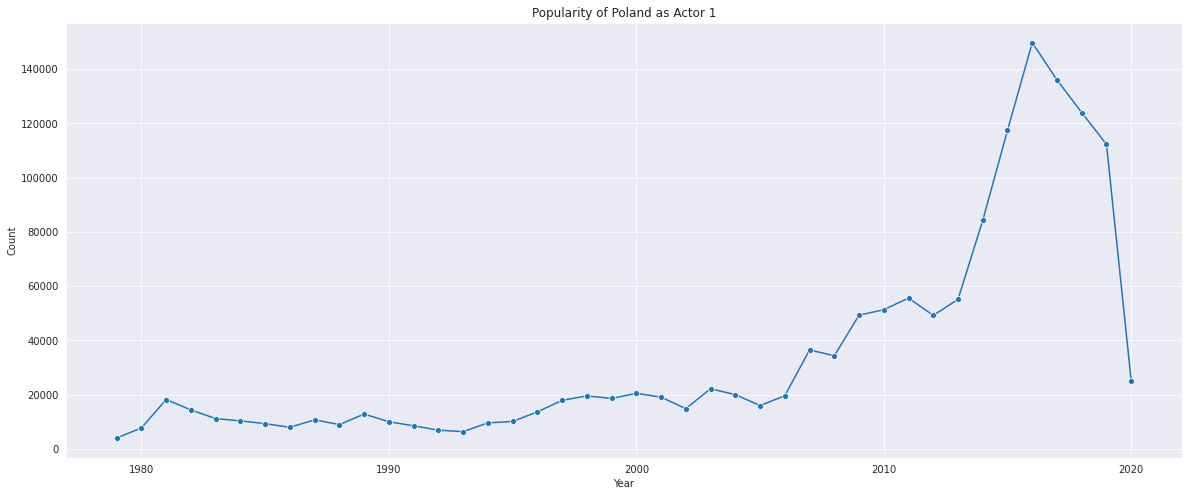
\includegraphics[width=1 \textwidth]{fig/PL/PLactor1.png}
        \caption{Liczba zdarzeń z Polską jako aktorem 1. (źródło: opracowanie własne)}
        \label{fig:PLactor1}
        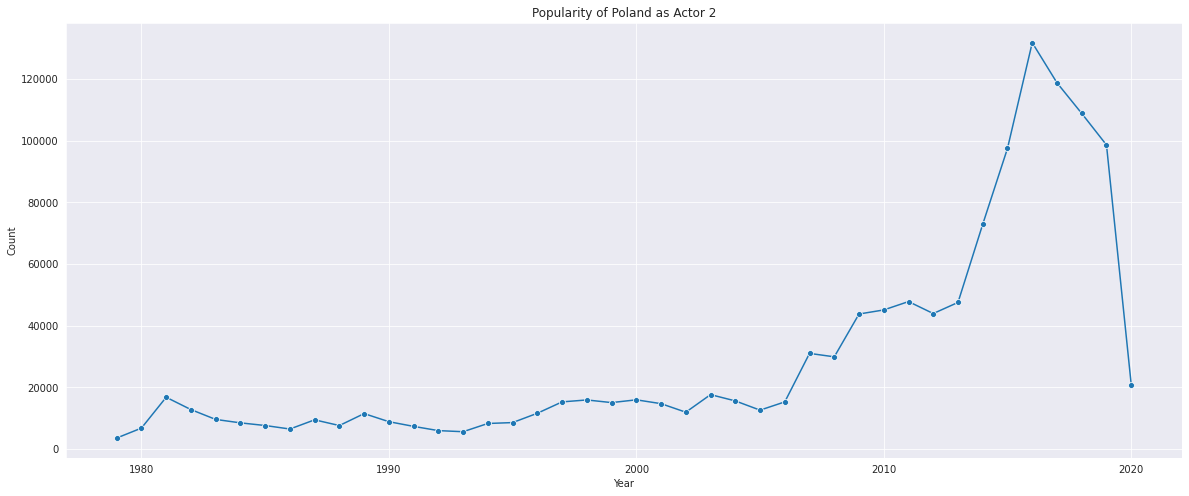
\includegraphics[width=1 \textwidth]{fig/PL/PLactor2.png}
        \caption{Liczba zdarzeń z Polską jako aktorem 2. (źródło: opracowanie własne)}
        \label{fig:PLactor2}
    \end{figure}

    \paragraph{Polska jako Aktor 2}
    Wykers~\ref{fig:PLactor2} przedstawia popularność Polski jako aktora 2 skumulowaną dla poszczególnych lat. Kształt wykresu jest bardzo zbliżony do~\ref{fig:PLactor1} jednak szczyt popularności jest niższy - na poziomie około 130 tysięcy zdarzeń.

    \paragraph{Polska jako miejsce wydarzeń}
    Wykers~\ref{fig:PLlocation} przedstawia popularność Polski jako miejsca wydarzeń skumulowaną dla poszczególnych lat. Ponownie kształt wykresu jest zbliżony do~\ref{fig:PLactor1}. W tym przypadku szczyt popularności jest wyższy - na poziomie około 210 tysięcy zdarzeń.
    \begin{figure}[ht!]
        \centering
        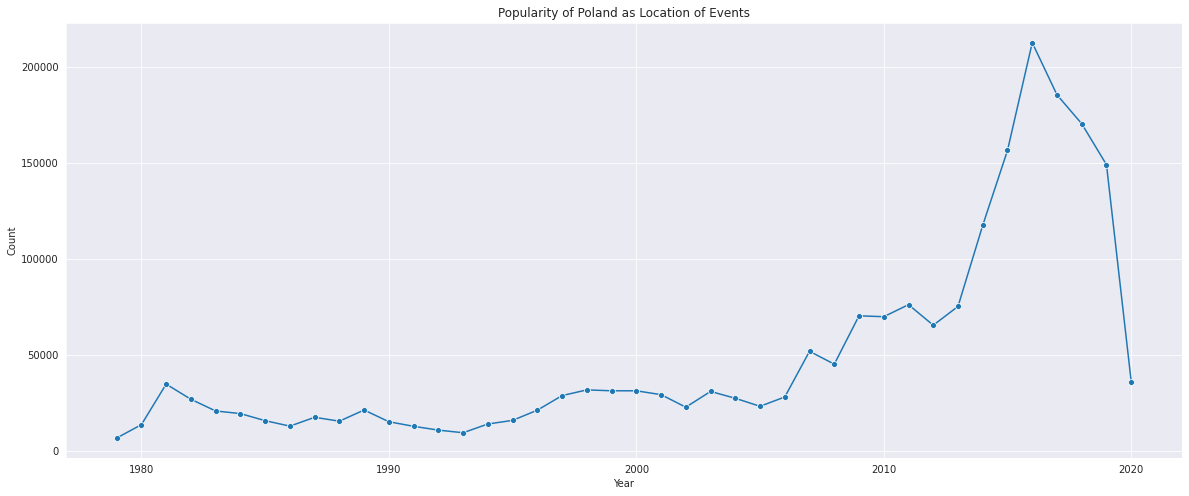
\includegraphics[width=1 \textwidth]{fig/PL/PLlocation.png}
        \caption{Liczba zdarzeń z Polską jako lokacją. (źródło: opracowanie własne)}
        \label{fig:PLlocation}
    \end{figure}

    \subsection{Analiza zbiorcza od 2015 roku}
    Dane pochodzą z przedziału od stycznia 2015 do kwietnia 2020 roku.

    \paragraph{Liczba zdarzeń dla poszczególnych krajów}
    Wykres~\ref{fig:GLOBALactor1} przedstawia sumaryczną liczbę zdarzeń od 2015 roku, dla poszczególnych krajów, uszeregowaną malejąco.
    \begin{figure}[ht!]
        \centering
        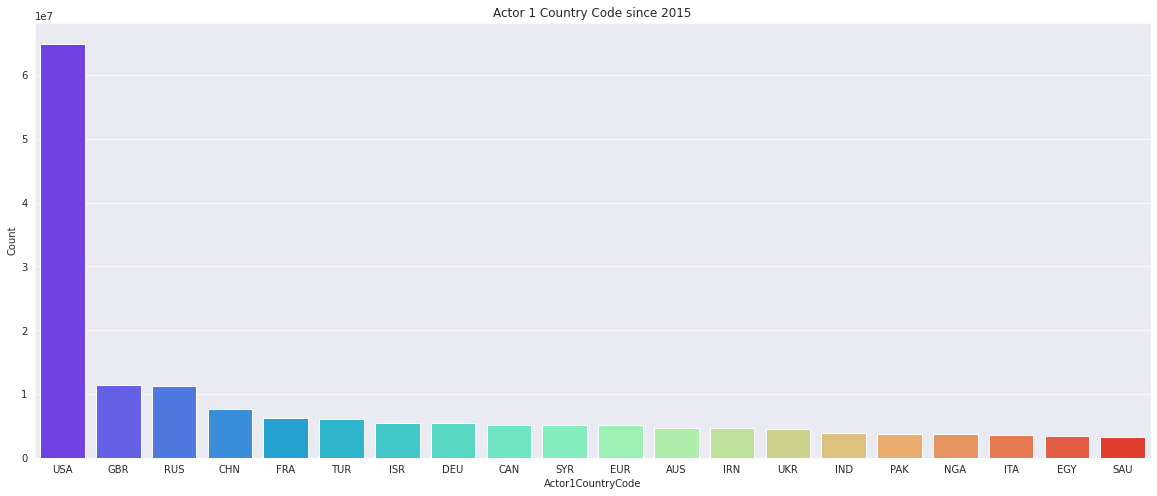
\includegraphics[width=1 \textwidth]{fig/GLOBAL/Actor1.png}
        \caption{Liczba zdarzeń dla poszczególnych krajów. (źródło: opracowanie własne)}
        \label{fig:GLOBALactor1}
    \end{figure}
    Niekwestionowanym liderem pod względem liczby zdarzeń są Stany Zjednoczone. Dystansują one pozostałe kraje o prawie rząd wielkości. Kraje anglosaskie są szczeegolnie mocno reprezentowane. W czołówce pojawiają sie też kraje znaczace polictycznie oraz silnie skonfliktowane.

    \paragraph{Liczba zdarzeń w czasie}
    Wykres~\ref{fig:GLOBALactor1inTime} przedstawia liczbę zdarzeń dla top 5 krajów skumulowaną dla poszczególnych lat.
    WYKRES DO POPRAWY
    \begin{figure}[ht!]
        \centering
        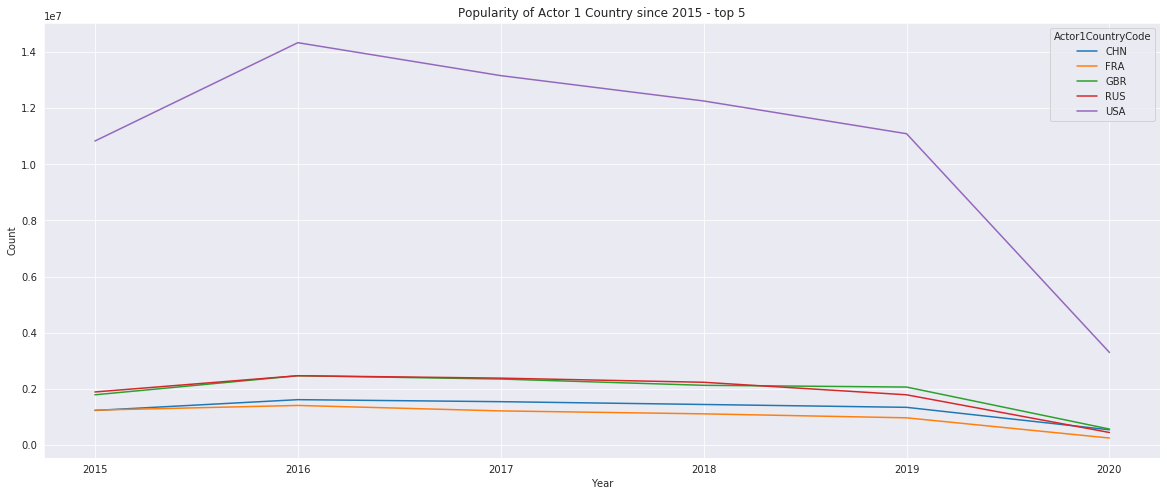
\includegraphics[width=1 \textwidth]{fig/GLOBAL/Actor1inTIME.png}
        \caption{Liczba zdarzeń dla poszczególnych krajów w czasie. (źródło: opracowanie własne)}
        \label{fig:GLOBALactor1inTime}
    \end{figure}

    \paragraph{Popularność czterokodów zdarzeń}
    Wykres~\ref{fig:GLOBALQC} przedstawia sumaryczną liczbę zdarzeń od 2015 roku, dla poszczególnych czterokodów zdarzeń, uszeregowaną malejąco.
    \begin{figure}[ht!]
        \centering
        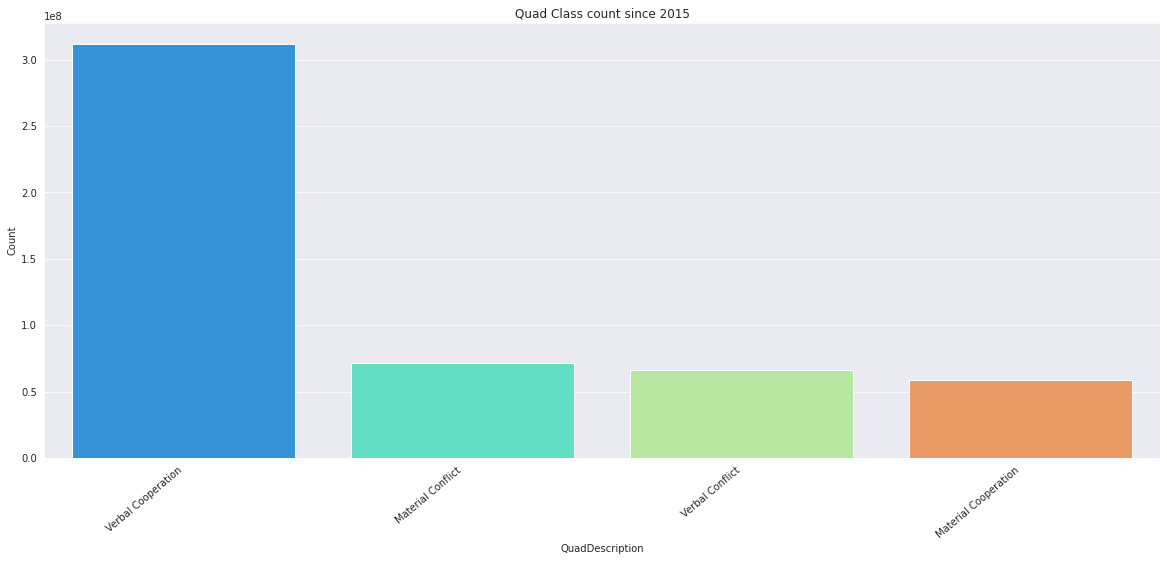
\includegraphics[width=1 \textwidth]{fig/GLOBAL/QC.png}
        \caption{Liczba zdarzeń dla poszczególnych kodów w czasie. (źródło: opracowanie własne)}
        \label{fig:GLOBALQC}
    \end{figure}

    \paragraph{Popularność czterokodów zdarzeń w czasie}
    Wykres~\ref{fig:GLOBALQCperc} przedstawia liczbę zdarzeń dla czterokodów zdarzeń skumulowaną dla poszczególnych lat.
    WYKRES DO POPRAWY
    \begin{figure}[ht!]
        \centering
        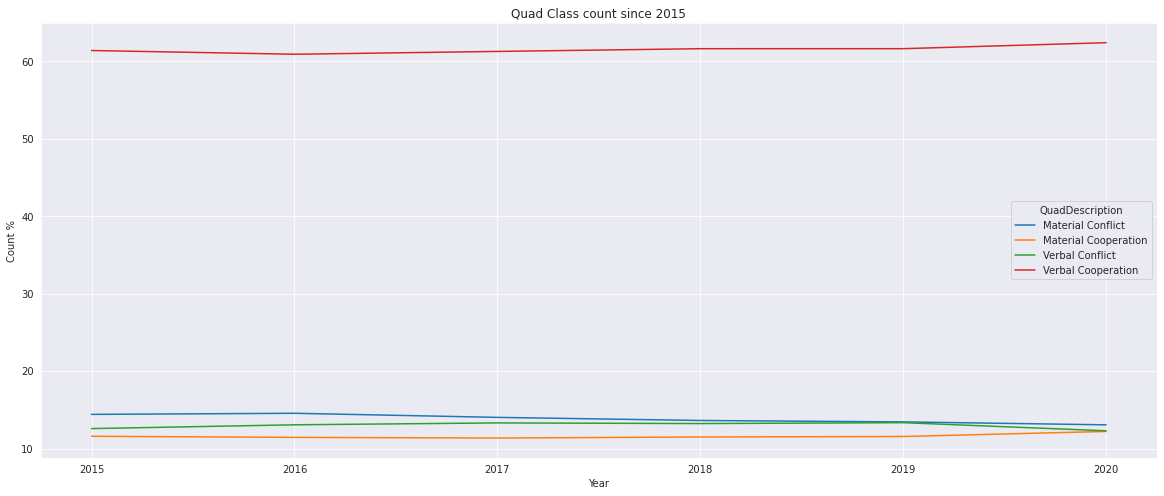
\includegraphics[width=1 \textwidth]{fig/GLOBAL/QCperc.png}
        \caption{Procentowa liczba zdarzeń dla poszczególnych kodów w czasie. (źródło: opracowanie własne)}
        \label{fig:GLOBALQCperc}
    \end{figure}

    \paragraph{Popularność bazowych kodów zdarzeń}
    Wykres~\ref{fig:GLOBALEBC} przedstawia sumaryczną liczbę zdarzeń od 2015 roku, dla poszczególnych bazowych kodów zdarzeń, uszeregowaną malejąco.
    \begin{figure}[ht!]
        \centering
        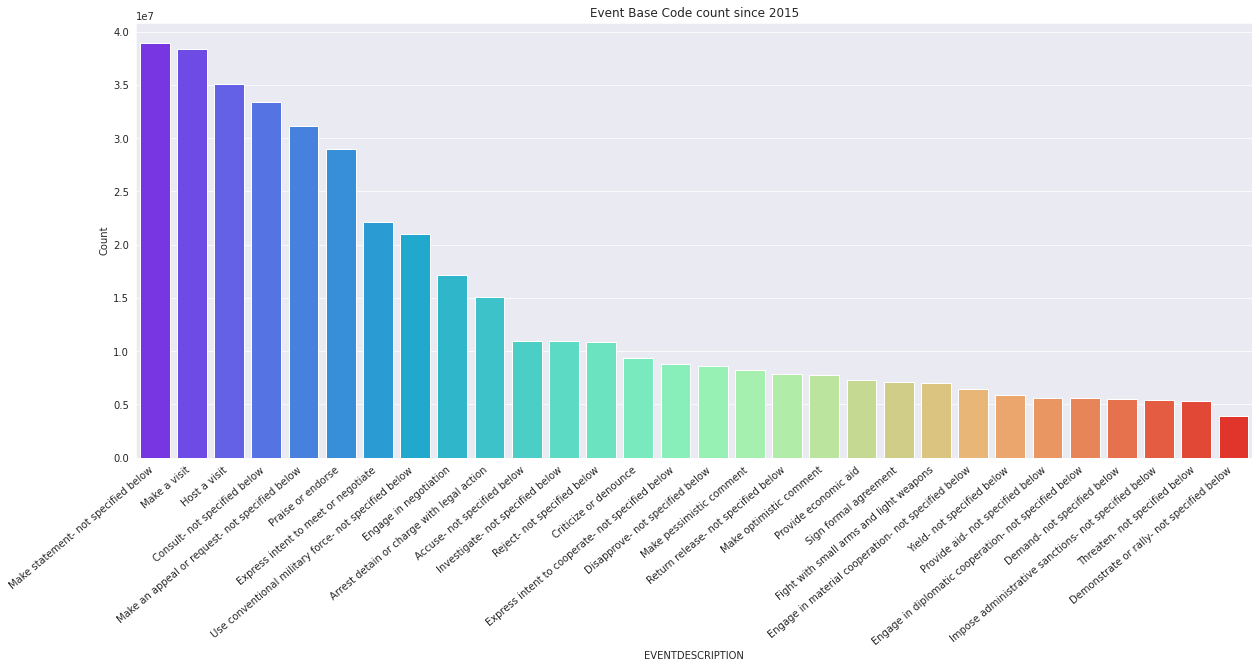
\includegraphics[width=1 \textwidth]{fig/GLOBAL/EBC.png}
        \caption{Liczba zdarzeń dla poszczególnych kodów w czasie. (źródło: opracowanie własne)}
        \label{fig:GLOBALEBC}
    \end{figure}

    \paragraph{Popularność bazowych kodów zdarzeń w czasie}
    Wykres~\ref{fig:GLOBALEBCperc} przedstawia liczbę zdarzeń dla top 20 bazowych kodów zdarzeń skumulowaną dla poszczególnych lat.
    WYKRES DO POPRAWY
    \begin{figure}[ht!]
        \centering
        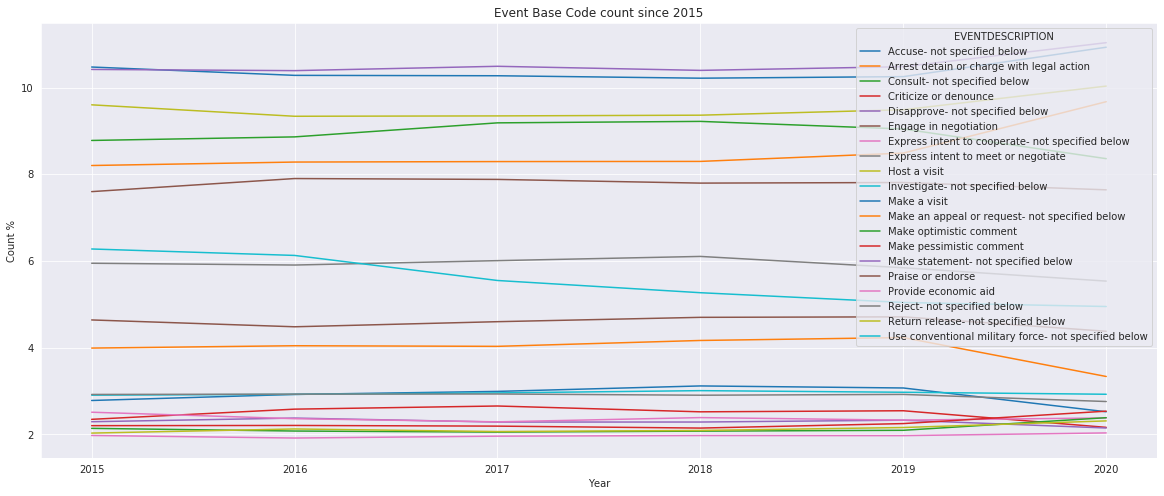
\includegraphics[width=1 \textwidth]{fig/GLOBAL/EBCperc.png}
        \caption{Procentowa liczba zdarzeń dla poszczególnych kodów w czasie. (źródło: opracowanie własne)}
        \label{fig:GLOBALEBCperc}
    \end{figure}

    \paragraph{Popularność podstawowych kodów zdarzeń}
    Wykres~\ref{fig:GLOBALERC} przedstawia sumaryczną liczbę zdarzeń od 2015 roku, dla poszczególnych podstawowych kodów zdarzeń, uszeregowaną malejąco.
    \begin{figure}[ht!]
        \centering
        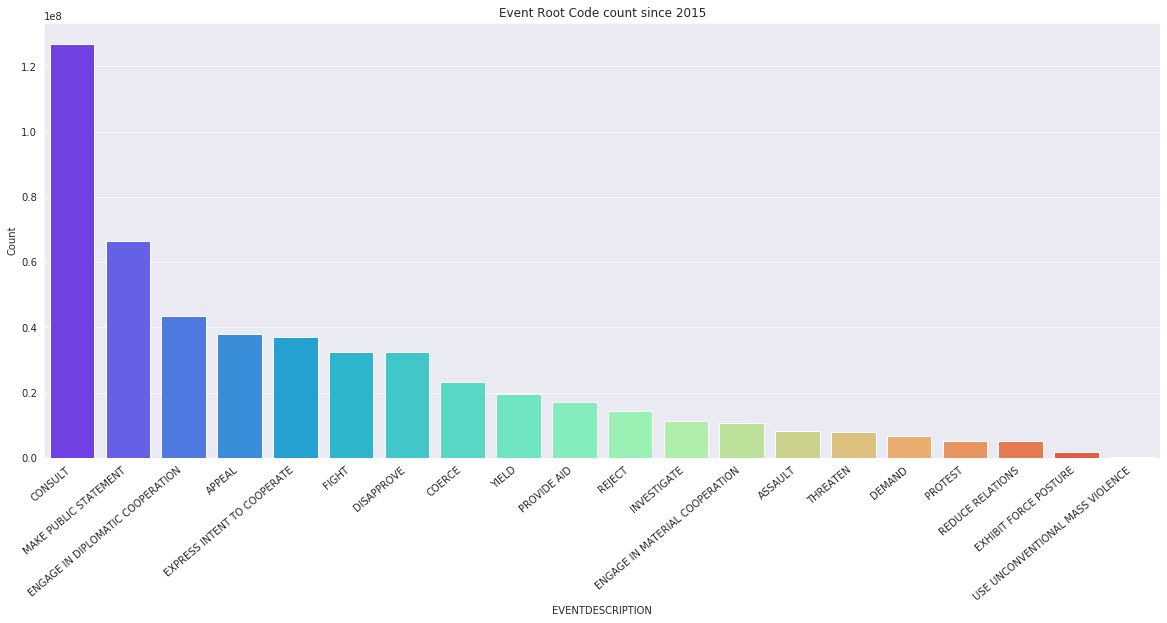
\includegraphics[width=1 \textwidth]{fig/GLOBAL/ERC.png}
        \caption{Liczba zdarzeń dla poszczególnych kodów w czasie. (źródło: opracowanie własne)}
        \label{fig:GLOBALERC}
    \end{figure}

    \paragraph{Popularność podstawowych kodów zdarzeń w czasie}
    Wykres~\ref{fig:GLOBALERCperc} przedstawia liczbę zdarzeń dla top 20 podstawowych kodów zdarzeń skumulowaną dla poszczególnych lat.
    WYKRES DO POPRAWY
    \begin{figure}[ht!]
        \centering
        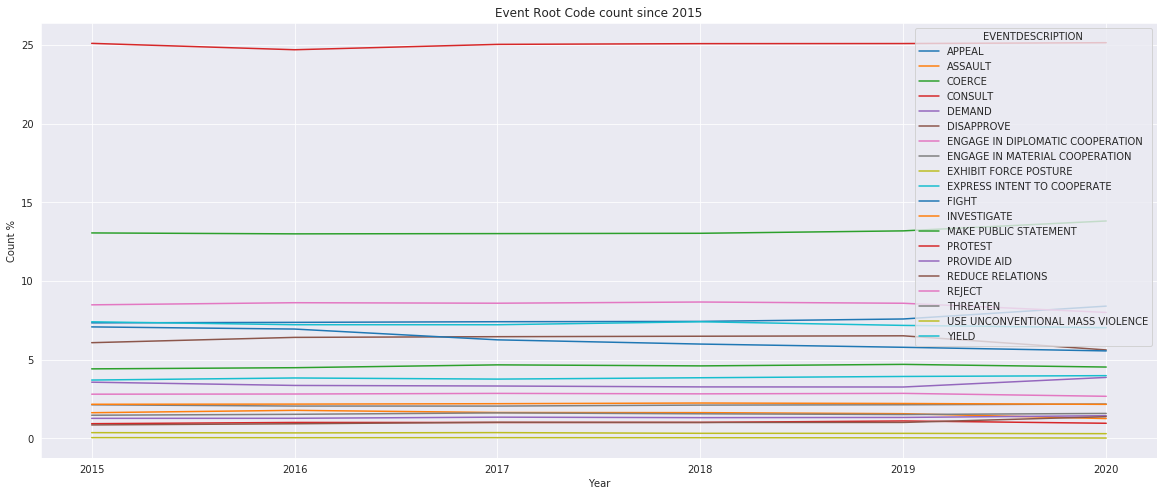
\includegraphics[width=1 \textwidth]{fig/GLOBAL/ERCperc.png}
        \caption{Procentowa liczba zdarzeń dla poszczególnych kodów w czasie. (źródło: opracowanie własne)}
        \label{fig:GLOBALERCperc}
    \end{figure}


    \section{Analiza danych dla wybranych krajów}

    \subsection{Polska}

    \paragraph{Kraj para do zdarzenia}


    Wykres~\ref{fig:PLpair} przedstawia liczbę zdarzeń dla Polski w których parą jest dany kraj.

    \begin{figure}[ht!]
        \centering
        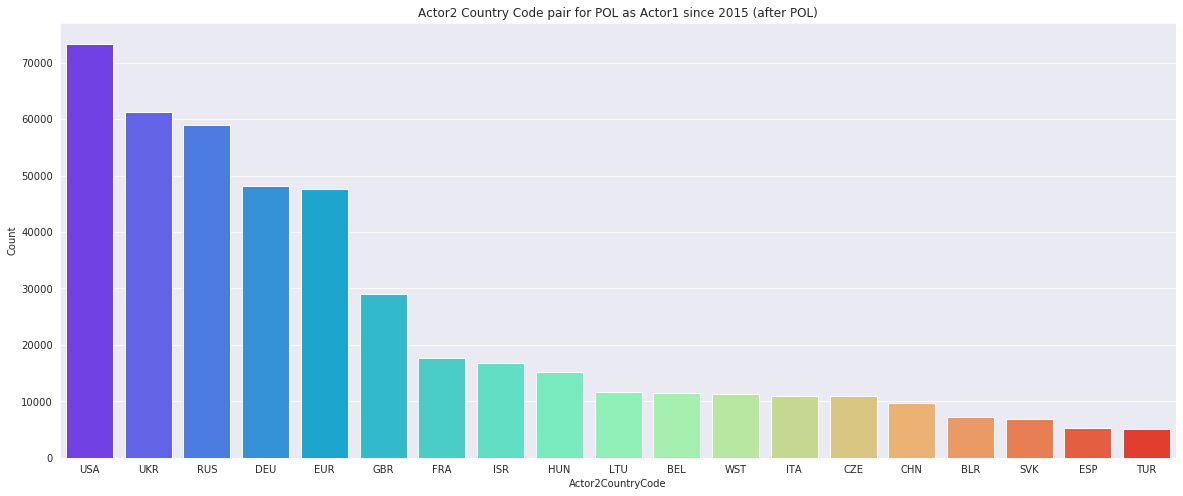
\includegraphics[width=1 \textwidth]{fig/PL/PLactor2Pair.png}
        \caption{Liczba zdarzeń w których parą jest dany kraj. (źródło: opracowanie własne)}
        \label{fig:PLpair}
    \end{figure}


    Wykres~\ref{fig:PLpairPerc} przedstawia liczbę zdarzeń dla Polski w których parą jest dany kraj w czasie.

    WYKRES DO POPRAWY
    \begin{figure}[ht!]
        \centering
        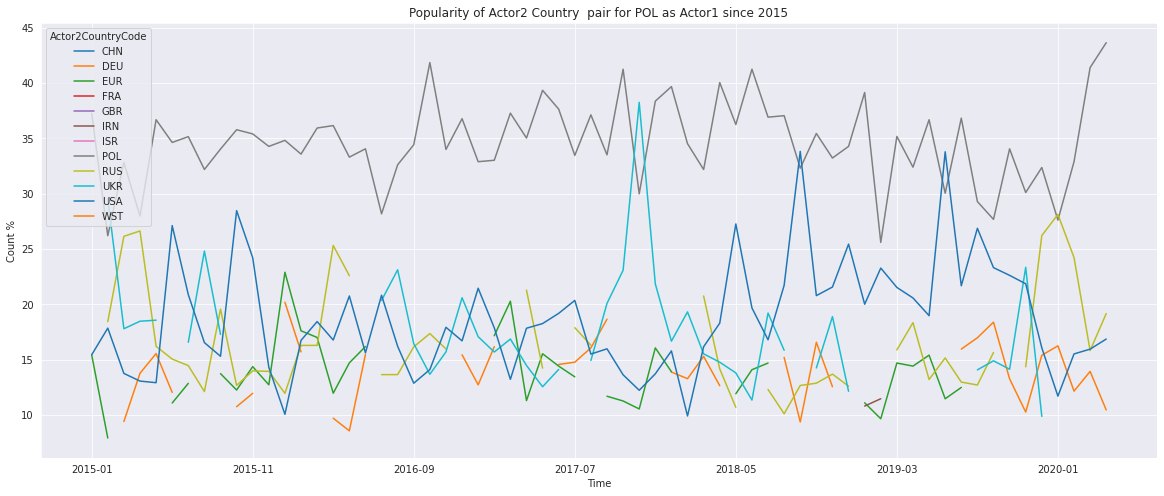
\includegraphics[width=1 \textwidth]{fig/PL/PLactor2PairPercinTIME.png}
        \caption{Procentowa liczba zdarzeń w których parą jest dany kraj w czasie. (źródło: opracowanie własne)}
        \label{fig:PLpairPerc}
    \end{figure}

    \paragraph{Podstawowy kod zdarzeń}

    Wykres~\ref{fig:PLPERC} przedstawia liczbę zdarzeń dla Polski dla poszczególnych kodów podstawowych.


    \begin{figure}[ht!]
        \centering
        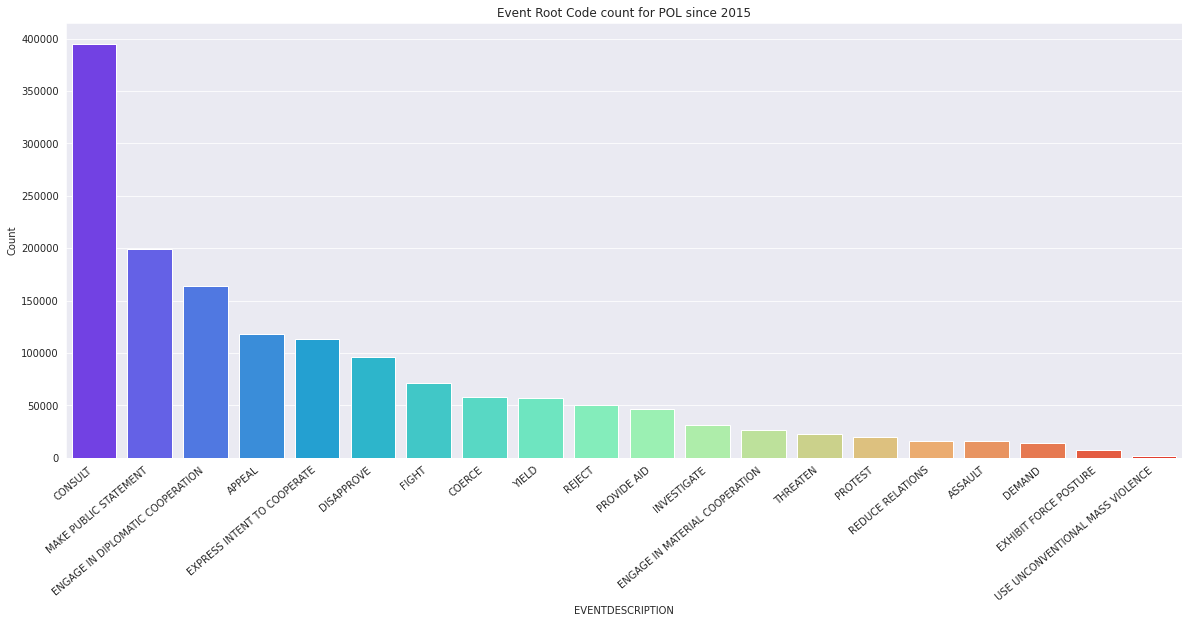
\includegraphics[width=1 \textwidth]{fig/PL/PLERC.png}
        \caption{Liczba zdarzeń dla poszczególnych kodów podstawowocy. (źródło: opracowanie własne)}
        \label{fig:PLPERC}
    \end{figure}

    Wykres~\ref{fig:PLPERCinTIME} przedstawia liczbę zdarzeń dla Polski dla poszczególnych kodów podstawowych w czasie.

    WYKRES DO POPRAWY
    \begin{figure}[ht!]
        \centering
        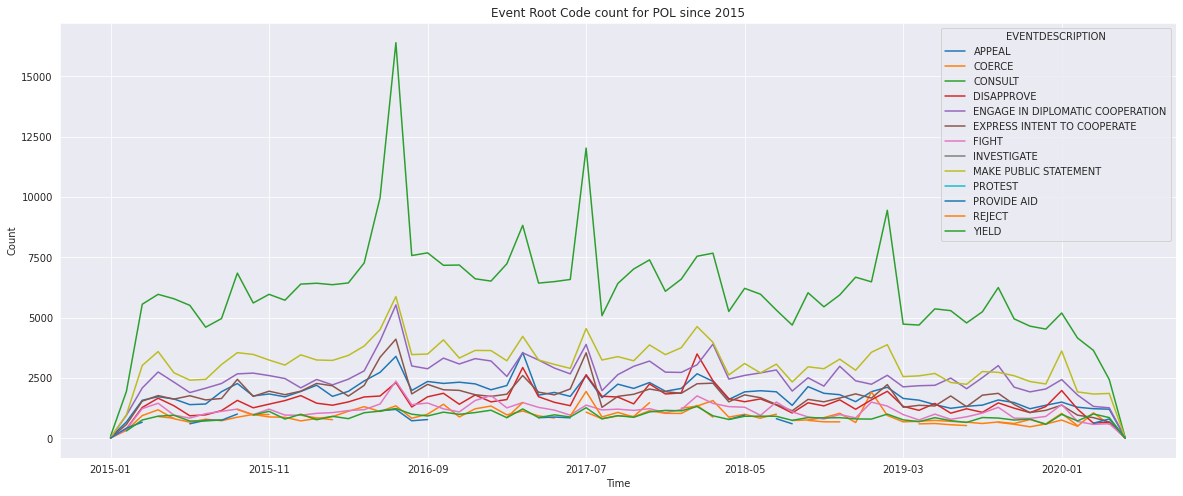
\includegraphics[width=1 \textwidth]{fig/PL/PLERCinTIME.png}
        \caption{Liczba zdarzeń dla poszczególnych kodów podstawowocy w czasie. (źródło: opracowanie własne)}
        \label{fig:PLPERCinTIME}
    \end{figure}

    Wykres~\ref{fig:PLPERCpercinTIME} przedstawia procentową liczbę zdarzeń dla Polski dla poszczególnych kodów podstawowych w czasie.

    WYKRES DO POPRAWY
    \begin{figure}[ht!]
        \centering
        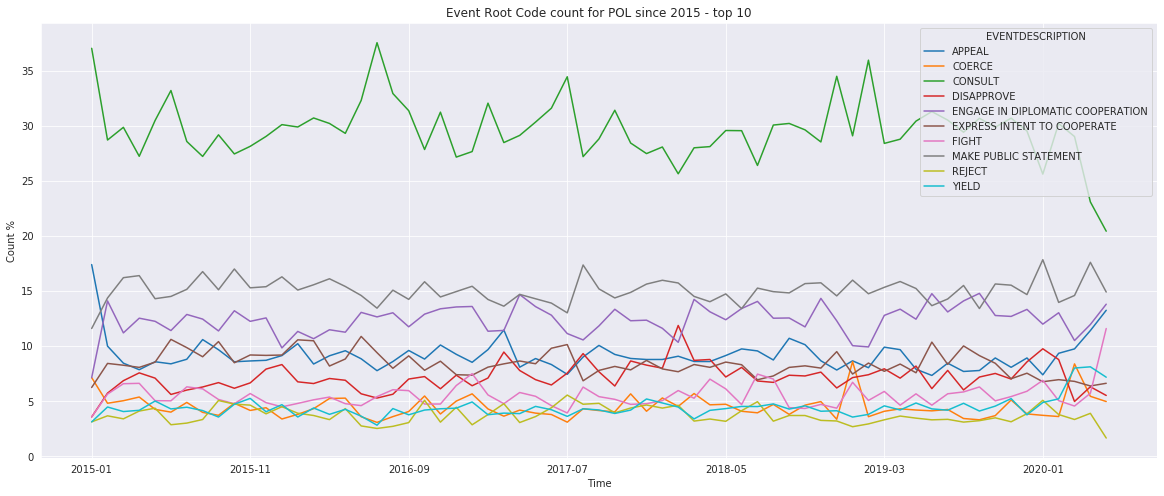
\includegraphics[width=1 \textwidth]{fig/PL/PLERCpercinTIME.png}
        \caption{Procentowa liczba zdarzeń dla poszczególnych kodów podstawowocy w czasie. (źródło: opracowanie własne)}
        \label{fig:PLPERCpercinTIME}
    \end{figure}

    \paragraph{Podstawowe kody zdarzeń między Polską a wybranymi krajami}

    Wykres~\ref{fig:PLDEUERC} przedstawia liczbę zdarzeń z Niemcami dla poszczególnych kodów podstawowocy w czasie.

    WYKRES DO POPRAWY
    \begin{figure}[ht!]
        \centering
        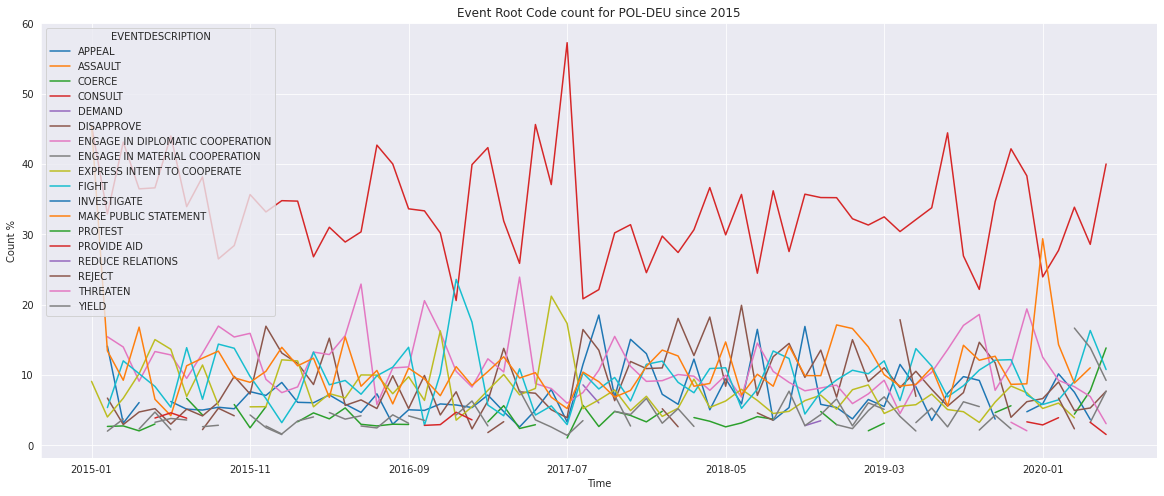
\includegraphics[width=1 \textwidth]{fig/PL/POLDEUERCperc.png}
        \caption{Procentowa liczba zdarzeń z Niemcami dla poszczególnych kodów podstawowocy w czasie. (źródło: opracowanie własne)}
        \label{fig:PLDEUERC}
    \end{figure}

    Wykres~\ref{fig:PLFRAERC} przedstawia liczbę zdarzeń z Francją dla poszczególnych kodów podstawowocy w czasie.


    WYKRES DO POPRAWY
    \begin{figure}[ht!]
        \centering
        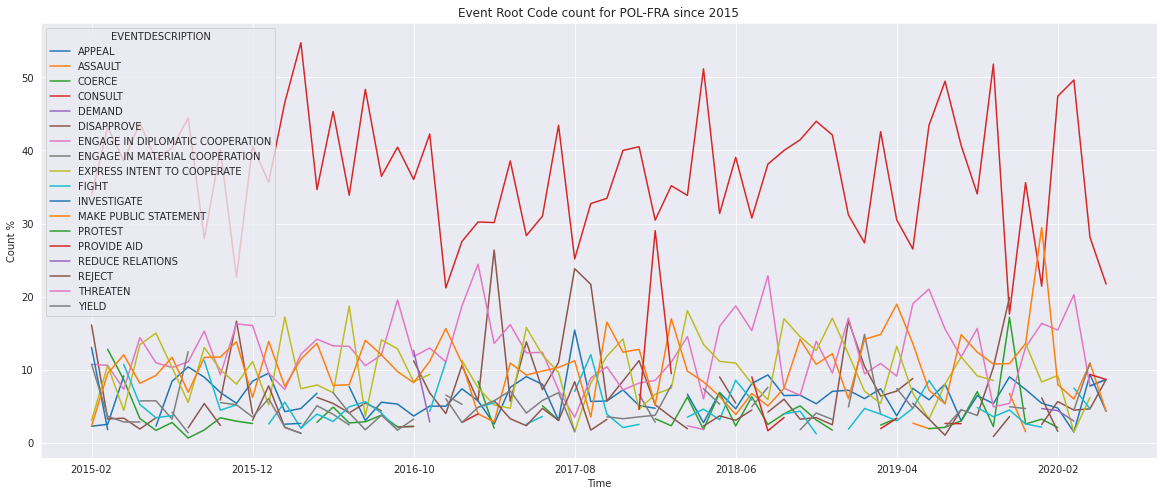
\includegraphics[width=1 \textwidth]{fig/PL/POLFRAERCperc.png}
        \caption{Procentowa liczba zdarzeń z Francją dla poszczególnych kodów podstawowocy w czasie. (źródło: opracowanie własne)}
        \label{fig:PLFRAERC}
    \end{figure}

    Wykres~\ref{fig:PLGBRERC} przedstawia liczbę zdarzeń z Wielką Brytanią dla poszczególnych kodów podstawowocy w czasie.

    WYKRES DO POPRAWY
    \begin{figure}[ht!]
        \centering
        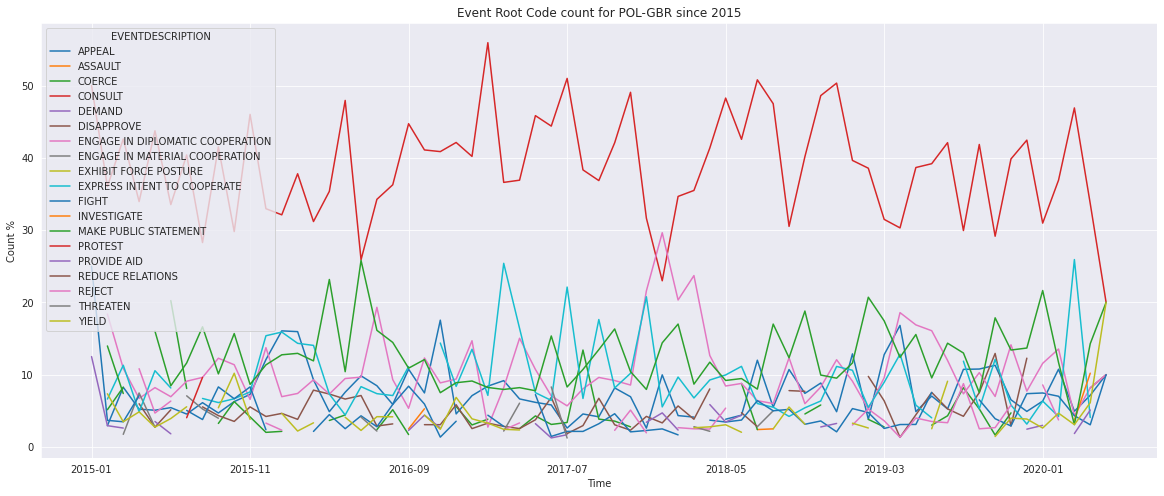
\includegraphics[width=1 \textwidth]{fig/PL/POLGBRERCperc.png}
        \caption{Procentowa liczba zdarzeń z Wielka Brytanią dla poszczególnych kodów podstawowocy w czasie. (źródło: opracowanie własne)}
        \label{fig:PLGBRERC}
    \end{figure}

    Wykres~\ref{fig:PLRUSERC} przedstawia liczbę zdarzeń z Rosją dla poszczególnych kodów podstawowocy w czasie.

    WYKRES DO POPRAWY
    \begin{figure}[ht!]
        \centering
        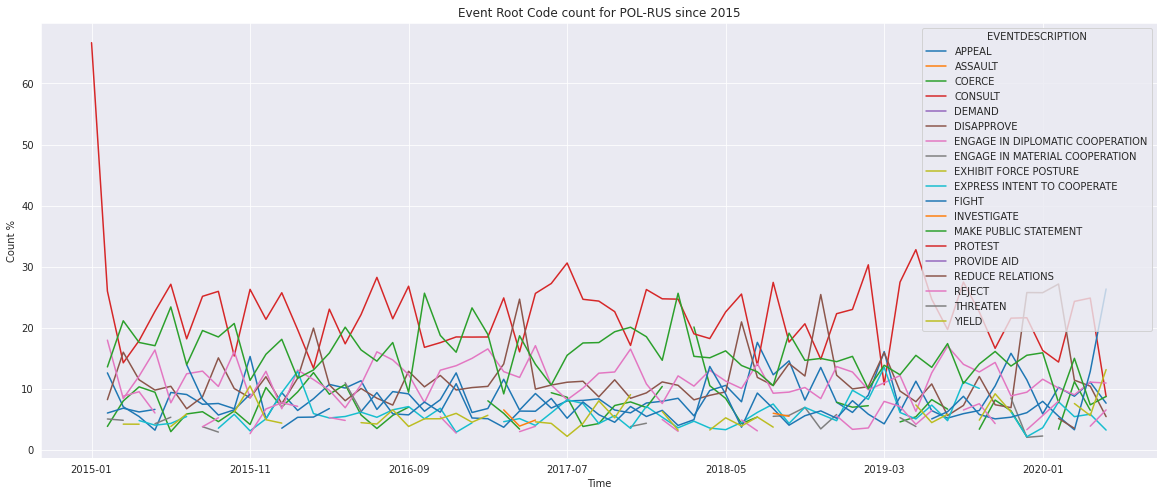
\includegraphics[width=1 \textwidth]{fig/PL/POLRUSERCperc.png}
        \caption{Procentowa liczba zdarzeń z Rosją dla poszczególnych kodów podstawowocy w czasie. (źródło: opracowanie własne)}
        \label{fig:PLRUSERC}
    \end{figure}

    \subsection{Niemcy}

    \subsection{Rosja}

    \subsection{Stan zjednoczone}

    \subsection{Pozostałe}


    \section{Analiza siły powiązania}

    \subsection{Analiza siły powiązania miedzy wybranymi krajami}

    \paragraph{Polska}

    Wykres~\ref{fig:PLConnection} przedstawia siłę połączenia Polski z wybranaymi krajami w czasie.


    \begin{figure}[ht!]
        \centering
        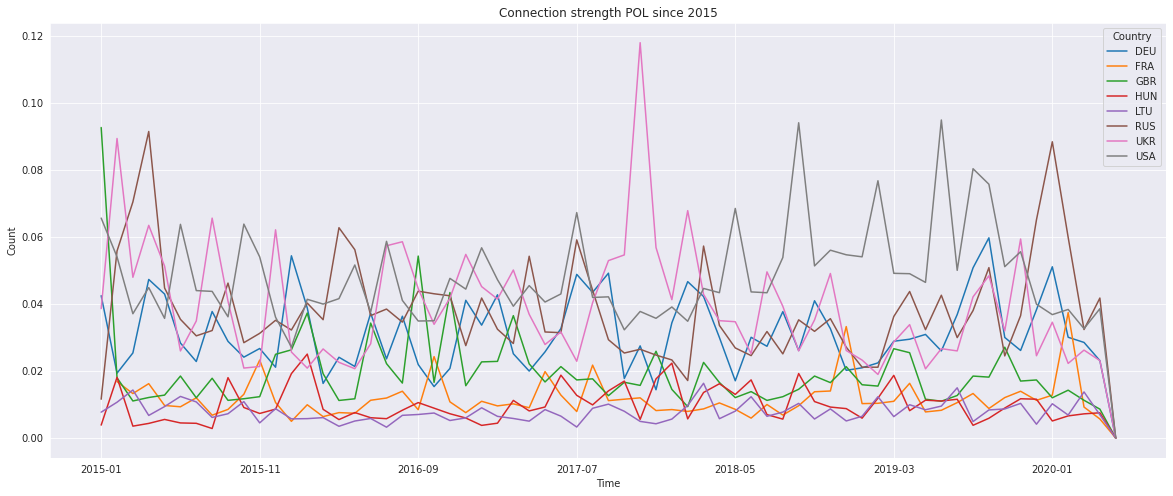
\includegraphics[width=1 \textwidth]{fig/PL/POLConnection.png}
        \caption{Siła połączenia Polski z wybranymi krajami w czasie. (źródło: opracowanie własne)}
        \label{fig:PLConnection}
    \end{figure}

    \paragraph{Rosja}

    Wykres~\ref{fig:RUSConnection} przedstawia siłę połączenia Rosji z wybranaymi krajami w czasie.

    \begin{figure}[ht!]
        \centering
        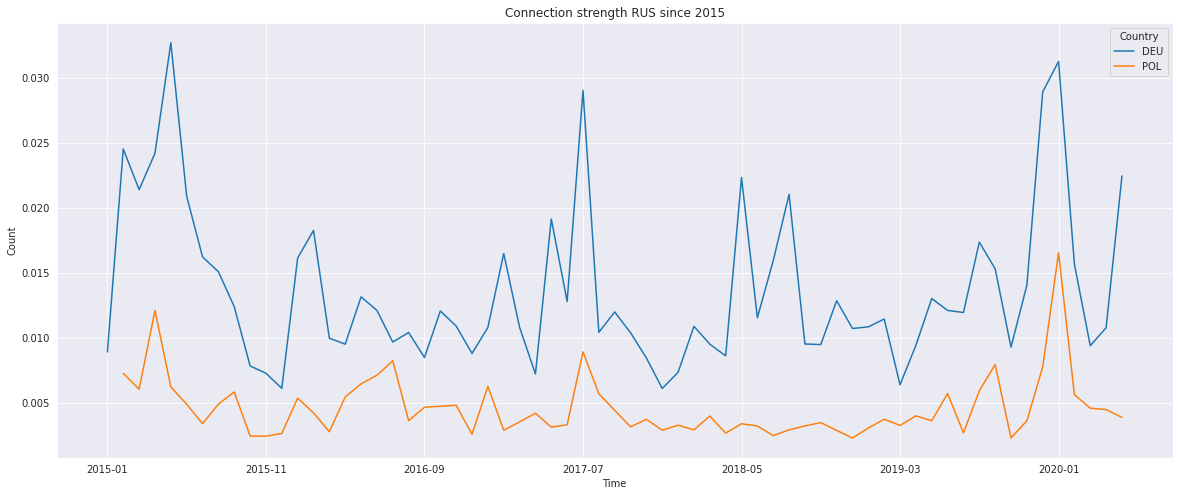
\includegraphics[width=1 \textwidth]{fig/RUS/RUSConnection.png}
        \caption{Siła połączenia Rosji z wybranymi krajami w czasie. (źródło: opracowanie własne)}
        \label{fig:RUSConnection}
    \end{figure}

    \paragraph{Niemcy}

    Wykres~\ref{fig:DEUConnection} przedstawia siłę połączenia Niemiec z wybranaymi krajami w czasie.

    \begin{figure}[ht!]
        \centering
        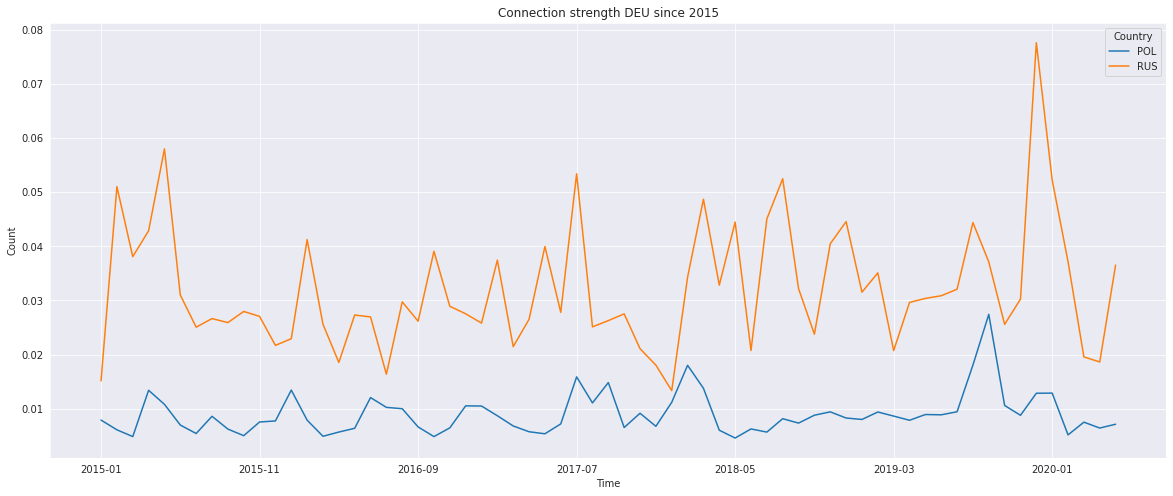
\includegraphics[width=1 \textwidth]{fig/DEU/DEUConnection.png}
        \caption{Siła połączenia Niemiec z wybranymi krajami w czasie. (źródło: opracowanie własne)}
        \label{fig:DEUConnection}
    \end{figure}

    \paragraph{Stany Zjednoczone}

    Wykres~\ref{fig:PLConnection} przedstawia siłę połączenia Stanów Zjednoczonych z wybranaymi krajami w czasie.

    \begin{figure}[ht!]
        \centering
        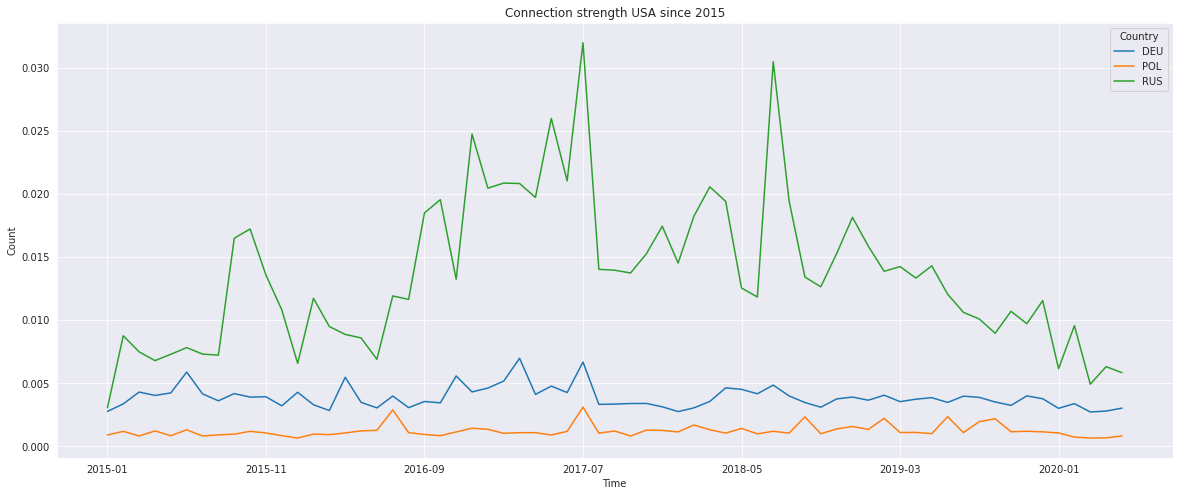
\includegraphics[width=1 \textwidth]{fig/USA/USAConnection.png}
        \caption{Siła połączenia Stanów Zjednoczonych z wybranymi krajami w czasie. (źródło: opracowanie własne)}
        \label{fig:USAConnection}
    \end{figure}

    \subsection{Analiza symetryczności siły powiązania}

    \paragraph{Polska - Niemcy - Polska}

    Wykres~\ref{fig:POL-DEU-POL} przedstawia symetryczność siły połączenia Polski i Niemiec w czasie.


    \begin{figure}[ht!]
        \centering
        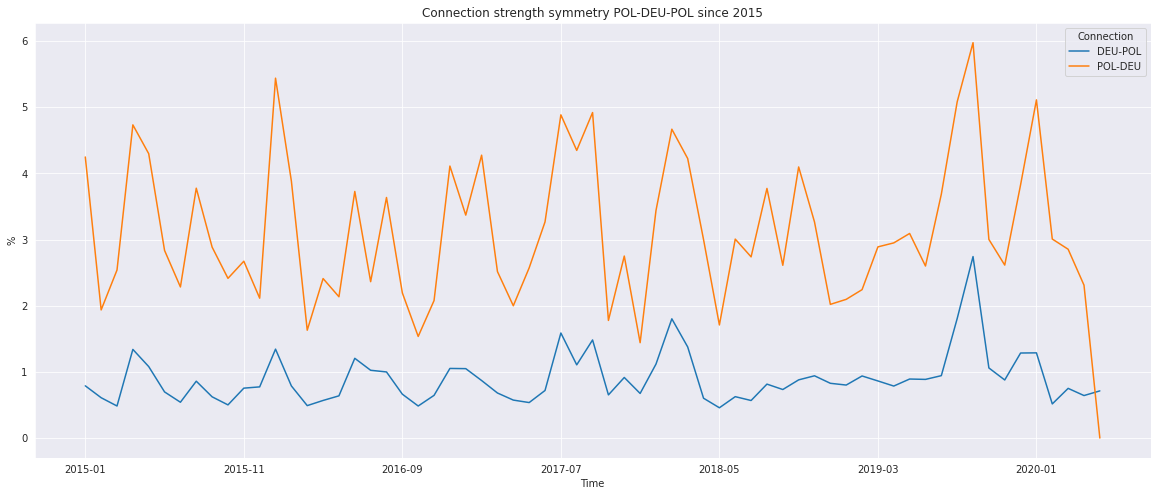
\includegraphics[width=1 \textwidth]{fig/ConnectionSymmetry/POL-DEU-POL.png}
        \caption{Symetryczność siły połączenia Polski i Niemiec w czasie. (źródło: opracowanie własne)}
        \label{fig:POL-DEU-POL}
    \end{figure}

    \paragraph{Polska - Rosja - Polska}

    Wykres~\ref{fig:POL-RUS-POL} przedstawia symetryczność siły połączenia Polski i Rosji w czasie.


    \begin{figure}[ht!]
        \centering
        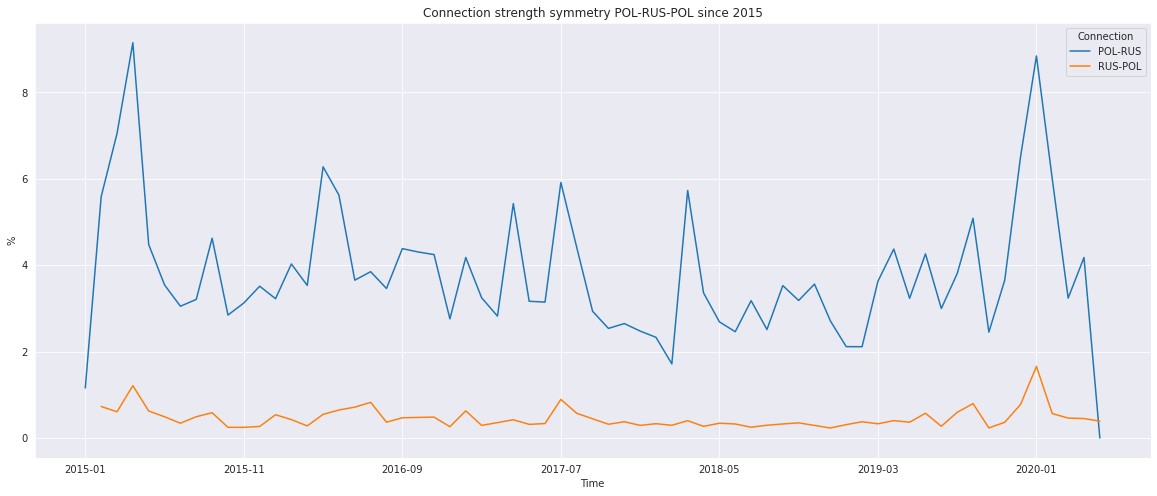
\includegraphics[width=1 \textwidth]{fig/ConnectionSymmetry/POL-RUS-POL.png}
        \caption{Symetryczność siły połączenia Polski i Rosji w czasie. (źródło: opracowanie własne)}
        \label{fig:POL-RUS-POL}
    \end{figure}

    \paragraph{Polska - Stany Zjednoczone - Polska}

    Wykres~\ref{fig:POL-USA-POL} przedstawia symetryczność siły połączenia Polski i Stanów Zjednoczonych w czasie.


    \begin{figure}[ht!]
        \centering
        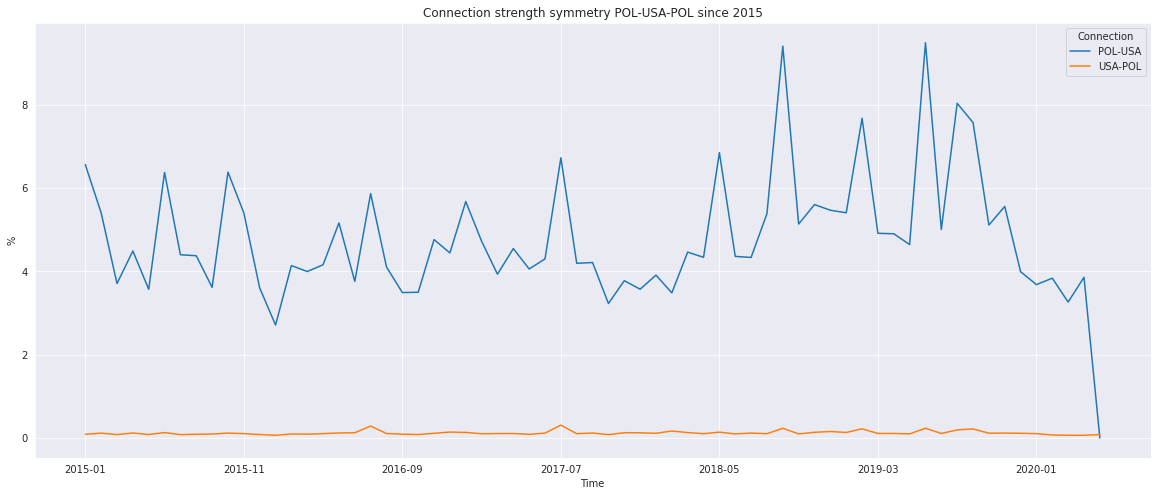
\includegraphics[width=1 \textwidth]{fig/ConnectionSymmetry/POL-USA-POL.png}
        \caption{Symetryczność siły połączenia Polski i Stanów Zjednoczonych w czasie. (źródło: opracowanie własne)}
        \label{fig:POL-USA-POL}
    \end{figure}


    \section{Analiza wybranych kodów podstawowych}

    \subsection{Fight}

    Wykres~\ref{fig:Fight} przedstawia procentową liczbę państw z jakimi dany kraj ma zdarzenia fight w czasie.


    \begin{figure}[ht!]
        \centering
        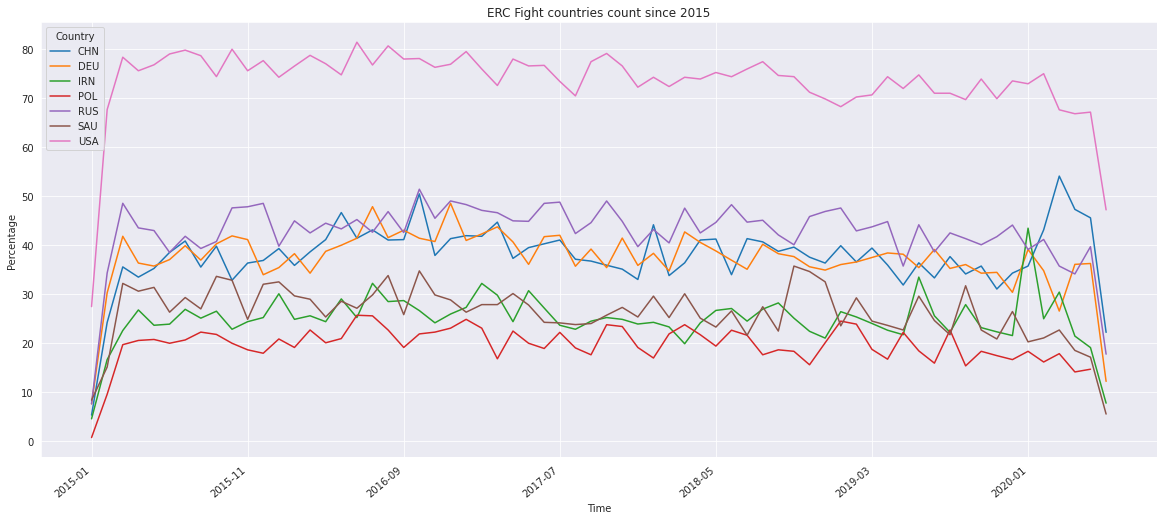
\includegraphics[width=1 \textwidth]{fig/ERC/Fight.png}
        \caption{Procentowa liczba państw z jakimi dany kraj ma zdarzenia fight w czasie. (źródło: opracowanie własne)}
        \label{fig:Fight}
    \end{figure}

    \subsection{Express intent to cooperate}

    Wykres\ldots przedstawia procentową liczbę państw z jakimi dany kraj ma zdarzenia fight w czasie.


    \section{Analiza średniego tonu wydarzeń dla wybranych krajów}


    \section{Analiza miary Goldsteina wydarzeń dla wybranych krajów}


    \section{Klasteryzacja}

    \subsection{Grupowanie z wykorzystaniem K-Means - 10 klastrów}

    Do przeprowadzenia pierwszego grupowania krajów wykorzystany został wektor składający się z:
    \begin{enumerate}
        \item[•] liczby zdarzeń dla których kraj jest aktorem 1
        \item[•] liczby wzmianek (numMentions)
        \item[•] stosunku liczby zdarzeń material conflict do material cooperation z quad description
        \item[•] stosunku liczby zdarzeń verbal conflict do verbal cooperation z quad description
        \item[•] średniego średniego tonu
        \item[•] średniej miary Goldsteina
        \item[•] liczby zdarzeń Fight
        \item[•] liczby zdarzeń Express intent to cooperate
    \end{enumerate}
    Dane wykorzystane w tym doświadczeniu pochodzą ze stycznia 2020 roku.
    Przed dokonaniem klasteryzacji odrzucone zostały wydarzenia z kodami krajów cameo niezgodnymi z kodami ISO 3166-1 alfa-3~\cite{iso_alfa3}.
    Klasteryzacja została przeprowadzona dwukrotnie, za drugim razem na danych ustandaryzowanych przy pomocy modułu StandardScaler~\cite{standardScaler}.

    \subsubsection{Dane niestandaryzowane}
    W pierwszej kolejności zostaną przedstawione wyniki grupowania na danych niestandaryzowanych.

    Wykres~\ref{fig:clust10} przedstawia mapę z naniesionymi wynikami klasteryzacji. Każda grupa krajów otrzymała inny kolor.

    \begin{figure}[ht!]
        \centering
        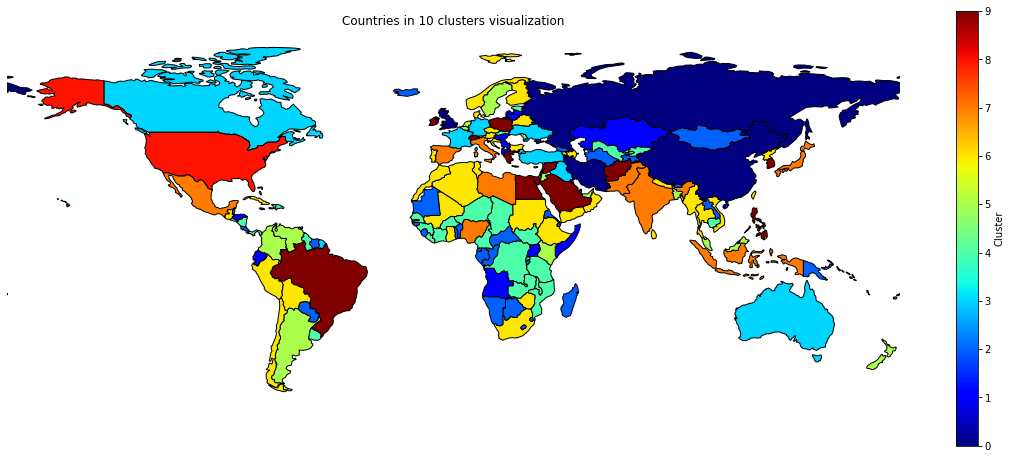
\includegraphics[width=1 \textwidth]{fig/CLUST/10clusterMap.png}
        \caption{Mapa z wynikami klasteryzacji. (źródło: opracowanie własne)}
        \label{fig:clust10}
    \end{figure}

    \paragraph{Wyniki klasteryzacji w postaci tabelarycznej}
    W tabelach od~\ref{tab:cl0} do~\ref{tab:cl9} przedstawione zostały wyniki grupowania.
    Dodatkowo zawarto informacje o liczbie ludności i PKB na osobę pochodzące z biblioteki GeoPandas~\cite{geopandas}.

    \begin{table}[h!]
   \centering
   \caption{Klaster 0}
   \label{tab:cl0}
   \begin{tabular}{lllrr}
      \toprule
      iso\_a3 & name         & continent     & pop\_est  & gdp\_per\_cap \\
      \midrule
      DZA     & Algeria      & Africa        & 40969443  & 0.01487       \\
      ARM     & Armenia      & Asia          & 3045191   & 0.008637      \\
      AUT     & Austria      & Europe        & 8754413   & 0.04759       \\
      AZE     & Azerbaijan   & Asia          & 9961396   & 0.01686       \\
      BLR     & Belarus      & Europe        & 9549747   & 0.01732       \\
      BOL     & Bolivia      & South America & 11138234  & 0.007034      \\
      BGR     & Bulgaria     & Europe        & 7101510   & 0.02015       \\
      CHL     & Chile        & South America & 17789267  & 0.02451       \\
      HRV     & Croatia      & Europe        & 4292095   & 0.02196       \\
      CUB     & Cuba         & North America & 11147407  & 0.01192       \\
      CYP     & Cyprus       & Asia          & 1221549   & 0.02395       \\
      CYP     & Cyprus       & Asia          & 1221549   & 0.02395       \\
      CZE     & Czechia      & Europe        & 10674723  & 0.03287       \\
      DNK     & Denmark      & Europe        & 5605948   & 0.04724       \\
      ETH     & Ethiopia     & Africa        & 105350020 & 0.001658      \\
      FIN     & Finland      & Europe        & 5491218   & 0.04082       \\
      GHA     & Ghana        & Africa        & 27499924  & 0.004393      \\
      GTM     & Guatemala    & North America & 15460732  & 0.008525      \\
      MLI     & Mali         & Africa        & 17885245  & 0.00213       \\
      MAR     & Morocco      & Africa        & 33986655  & 0.008321      \\
      MMR     & Myanmar      & Asia          & 55123814  & 0.005644      \\
      CYP     & N. Cyprus    & Asia          & 265100    & 0.01358       \\
      CYP     & N. Cyprus    & Asia          & 265100    & 0.01358       \\
      NPL     & Nepal        & Asia          & 29384297  & 0.002434      \\
      PRK     & North Korea  & Asia          & 25248140  & 0.001584      \\
      NOR     & Norway       & Europe        & 5320045   & 0.06855       \\
      OMN     & Oman         & Asia          & 3424386   & 0.05055       \\
      PER     & Peru         & South America & 31036656  & 0.01322       \\
      PRT     & Portugal     & Europe        & 10839514  & 0.02741       \\
      ZAF     & South Africa & Africa        & 54841552  & 0.01348       \\
      LKA     & Sri Lanka    & Asia          & 22409381  & 0.01056       \\
      SDN     & Sudan        & Africa        & 37345935  & 0.004721      \\
      TWN     & Taiwan       & Asia          & 23508428  & 0.04794       \\
      THA     & Thailand     & Asia          & 68414135  & 0.01697       \\
      TUN     & Tunisia      & Africa        & 11403800  & 0.01147       \\
      VNM     & Vietnam      & Asia          & 96160163  & 0.006187      \\
      YEM     & Yemen        & Asia          & 28036829  & 0.00262       \\
      ZWE     & Zimbabwe     & Africa        & 13805084  & 0.002052      \\
      \bottomrule
   \end{tabular}
\end{table}

    \begin{table}
    \centering
    \caption{Klaster 1}
    \label{tab:cl1}
    \begin{tabular}{llllr}
        \toprule
        iso\_a3 & name                 & continent     & pop\_est    & gdp\_per\_cap \\
        \midrule
        ARG     & Argentina            & South America & 44,293,293  & 0.02          \\
        BGD     & Bangladesh           & Asia          & 157,826,578 & 0.004         \\
        BEL     & Belgium              & Europe        & 11,491,346  & 0.044         \\
        COL     & Colombia             & South America & 47,698,524  & 0.014         \\
        JOR     & Jordan               & Asia          & 10,248,069  & 0.0084        \\
        KEN     & Kenya                & Africa        & 47,615,739  & 0.0032        \\
        LBN     & Lebanon              & Asia          & 6,229,794   & 0.014         \\
        MYS     & Malaysia             & Asia          & 31,381,992  & 0.027         \\
        NLD     & Netherlands          & Europe        & 17,084,719  & 0.051         \\
        NZL     & New Zealand          & Oceania       & 4,510,327   & 0.039         \\
        SWE     & Sweden               & Europe        & 9,960,487   & 0.05          \\
        ARE     & United Arab Emirates & Asia          & 6,072,475   & 0.11          \\
        VEN     & Venezuela            & South America & 31,304,016  & 0.015         \\
        \bottomrule
    \end{tabular}
\end{table}

    \begin{table}[h!]
   \centering
   \caption{Klaster 2}
   \label{tab:cl2}
   \begin{tabular}{lllrr}
      \toprule
      iso\_a3 & name         & continent     & pop\_est  & gdp\_per\_cap \\
      \midrule
      AFG     & Afghanistan  & Asia          & 34124811  & 0.001878      \\
      BRA     & Brazil       & South America & 207353391 & 0.01486       \\
      EGY     & Egypt        & Africa        & 97041072  & 0.01139       \\
      GRC     & Greece       & Europe        & 10768477  & 0.02698       \\
      IRL     & Ireland      & Europe        & 5011102   & 0.06426       \\
      PSE     & Palestine    & Asia          & 4543126   & 0.004671      \\
      PHL     & Philippines  & Asia          & 104256076 & 0.007692      \\
      POL     & Poland       & Europe        & 38476269  & 0.02734       \\
      SAU     & Saudi Arabia & Asia          & 28571770  & 0.06058       \\
      KOR     & South Korea  & Asia          & 51181299  & 0.03769       \\
      CHE     & Switzerland  & Europe        & 8236303   & 0.06026       \\
      SYR     & Syria        & Asia          & 18028549  & 0.002789      \\
      \bottomrule
   \end{tabular}
\end{table}

    \begin{table}
    \centering
    \caption{Klaster 3}
    \label{tab:cl3}
    \begin{tabular}{llllr}
        \toprule
        iso\_a3 & name            & continent     & pop\_est   & gdp\_per\_cap \\
        \midrule
        BHS     & Bahamas         & North America & 329,988    & 0.027         \\
        BFA     & Burkina Faso    & Africa        & 20,107,509 & 0.0016        \\
        KHM     & Cambodia        & Asia          & 16,204,486 & 0.0036        \\
        CMR     & Cameroon        & Africa        & 24,994,885 & 0.0031        \\
        TCD     & Chad            & Africa        & 12,075,985 & 0.0025        \\
        CIV     & Côte d'Ivoire   & Africa        & 24,184,810 & 0.0036        \\
        COD     & Dem. Rep. Congo & Africa        & 83,301,151 & 0.00079       \\
        DOM     & Dominican Rep.  & North America & 10,734,247 & 0.015         \\
        SLV     & El Salvador     & North America & 6,172,011  & 0.0089        \\
        EST     & Estonia         & Europe        & 1,251,581  & 0.031         \\
        GMB     & Gambia          & Africa        & 2,051,363  & 0.0017        \\
        GIN     & Guinea          & Africa        & 12,413,867 & 0.0013        \\
        GUY     & Guyana          & South America & 737,718    & 0.0083        \\
        HTI     & Haiti           & North America & 10,646,714 & 0.0018        \\
        KGZ     & Kyrgyzstan      & Asia          & 5,789,122  & 0.0036        \\
        LBR     & Liberia         & Africa        & 4,689,021  & 0.00083       \\
        LUX     & Luxembourg      & Europe        & 594,130    & 0.099         \\
        MWI     & Malawi          & Africa        & 19,196,246 & 0.0011        \\
        MDA     & Moldova         & Europe        & 3,474,121  & 0.0053        \\
        MOZ     & Mozambique      & Africa        & 26,573,706 & 0.0013        \\
        NIC     & Nicaragua       & North America & 6,025,951  & 0.0056        \\
        NER     & Niger           & Africa        & 19,245,344 & 0.001         \\
        PAN     & Panama          & North America & 3,753,142  & 0.025         \\
        RWA     & Rwanda          & Africa        & 11,901,484 & 0.0018        \\
        SSD     & S. Sudan        & Africa        & 13,026,129 & 0.0016        \\
        SEN     & Senegal         & Africa        & 14,668,522 & 0.0027        \\
        SVK     & Slovakia        & Europe        & 5,445,829  & 0.031         \\
        TZA     & Tanzania        & Africa        & 53,950,935 & 0.0028        \\
        URY     & Uruguay         & South America & 3,360,148  & 0.022         \\
        UZB     & Uzbekistan      & Asia          & 29,748,859 & 0.0068        \\
        ZMB     & Zambia          & Africa        & 15,972,000 & 0.0041        \\
        \bottomrule
    \end{tabular}
\end{table}

    \begin{table}
    \centering
    \caption{Klaster 4}
    \label{tab:cl4}
    \begin{tabular}{llllr}
        \toprule
        iso\_a3 & name      & continent     & pop\_est      & gdp\_per\_cap \\
        \midrule
        IND     & India     & Asia          & 1,281,935,911 & 0.0068        \\
        IDN     & Indonesia & Asia          & 260,580,739   & 0.012         \\
        ITA     & Italy     & Europe        & 62,137,802    & 0.036         \\
        JPN     & Japan     & Asia          & 126,451,398   & 0.039         \\
        LBY     & Libya     & Africa        & 6,653,210     & 0.014         \\
        MEX     & Mexico    & North America & 124,574,795   & 0.019         \\
        NGA     & Nigeria   & Africa        & 190,632,261   & 0.0057        \\
        PAK     & Pakistan  & Asia          & 204,924,861   & 0.0048        \\
        ESP     & Spain     & Europe        & 48,958,159    & 0.035         \\
        \bottomrule
    \end{tabular}
\end{table}

    \begin{table}
    \centering
    \caption{Klaster 5}
    \label{tab:cl5}
    \begin{tabular}{llllr}
        \toprule
        iso\_a3 & name       & continent     & pop\_est   & gdp\_per\_cap \\
        \midrule
        ALB     & Albania    & Europe        & 3,047,987  & 0.011         \\
        AGO     & Angola     & Africa        & 29,310,273 & 0.0064        \\
        ECU     & Ecuador    & South America & 16,290,913 & 0.011         \\
        HND     & Honduras   & North America & 9,038,741  & 0.0048        \\
        HUN     & Hungary    & Europe        & 9,850,845  & 0.027         \\
        JAM     & Jamaica    & North America & 2,990,561  & 0.0085        \\
        KAZ     & Kazakhstan & Asia          & 18,556,698 & 0.025         \\
        KWT     & Kuwait     & Asia          & 2,875,422  & 0.1           \\
        LVA     & Latvia     & Europe        & 1,944,643  & 0.026         \\
        LTU     & Lithuania  & Europe        & 2,823,859  & 0.03          \\
        MKD     & Macedonia  & Europe        & 2,103,721  & 0.014         \\
        QAT     & Qatar      & Asia          & 2,314,307  & 0.14          \\
        SRB     & Serbia     & Europe        & 7,111,024  & 0.014         \\
        SOM     & Somalia    & Africa        & 7,531,386  & 0.00063       \\
        UGA     & Uganda     & Africa        & 39,570,125 & 0.0021        \\
        \bottomrule
    \end{tabular}
\end{table}

    \begin{table}
    \centering
    \caption{Klaster 6}
    \label{tab:cl6}
    \begin{tabular}{llllr}
        \toprule
        iso\_a3 & name           & continent & pop\_est      & gdp\_per\_cap \\
        \midrule
        CHN     & China          & Asia      & 1,379,302,771 & 0.015         \\
        IRN     & Iran           & Asia      & 82,021,564    & 0.018         \\
        RUS     & Russia         & Europe    & 142,257,519   & 0.026         \\
        GBR     & United Kingdom & Europe    & 64,769,452    & 0.043         \\
        \bottomrule
    \end{tabular}
\end{table}

    \begin{table}
    \centering
    \caption{Klaster 7}
    \label{tab:cl7}
    \begin{tabular}{llllr}
        \toprule
        iso\_a3 & name                     & continent     & pop\_est    & gdp\_per\_cap \\
        \midrule
        USA     & United States of America & North America & 326,625,791 & 0.057         \\
        \bottomrule
    \end{tabular}
\end{table}

    \begin{table}[h!]
   \centering
   \caption{Klaster 8}
   \label{tab:cl8}
   \begin{tabular}{lllrr}
      \toprule
      iso\_a3 & name                 & continent     & pop\_est & gdp\_per\_cap \\
      \midrule
      BLZ     & Belize               & North America & 360346   & 0.00857       \\
      BEN     & Benin                & Africa        & 11038805 & 0.002202      \\
      BTN     & Bhutan               & Asia          & 758288   & 0.008482      \\
      BWA     & Botswana             & Africa        & 2214858  & 0.01621       \\
      BRN     & Brunei               & Asia          & 443593   & 0.07604       \\
      BDI     & Burundi              & Africa        & 11466756 & 0.0006883     \\
      CAF     & Central African Rep. & Africa        & 5625118  & 0.0005699     \\
      COG     & Congo                & Africa        & 4954674  & 0.006109      \\
      CRI     & Costa Rica           & North America & 4930258  & 0.01608       \\
      DJI     & Djibouti             & Africa        & 865267   & 0.003866      \\
      GNQ     & Eq. Guinea           & Africa        & 778358   & 0.04082       \\
      ERI     & Eritrea              & Africa        & 5918919  & 0.001549      \\
      FJI     & Fiji                 & Oceania       & 920938   & 0.009093      \\
      GAB     & Gabon                & Africa        & 1772255  & 0.0203        \\
      GEO     & Georgia              & Asia          & 4926330  & 0.007565      \\
      GNB     & Guinea-Bissau        & Africa        & 1792338  & 0.001591      \\
      ISL     & Iceland              & Europe        & 339747   & 0.04754       \\
      LAO     & Laos                 & Asia          & 7126706  & 0.005747      \\
      LSO     & Lesotho              & Africa        & 1958042  & 0.003074      \\
      MDG     & Madagascar           & Africa        & 25054161 & 0.001471      \\
      MRT     & Mauritania           & Africa        & 3758571  & 0.004446      \\
      MNG     & Mongolia             & Asia          & 3068243  & 0.01206       \\
      NAM     & Namibia              & Africa        & 2484780  & 0.01046       \\
      PNG     & Papua New Guinea     & Oceania       & 6909701  & 0.004055      \\
      PRY     & Paraguay             & South America & 6943739  & 0.009313      \\
      SLE     & Sierra Leone         & Africa        & 6163195  & 0.001726      \\
      SLB     & Solomon Is.          & Oceania       & 647581   & 0.00185       \\
      SUR     & Suriname             & South America & 591919   & 0.01444       \\
      TJK     & Tajikistan           & Asia          & 8468555  & 0.003048      \\
      TGO     & Togo                 & Africa        & 7965055  & 0.001458      \\
      TTO     & Trinidad and Tobago  & North America & 1218208  & 0.03577       \\
      TKM     & Turkmenistan         & Asia          & 5351277  & 0.0177        \\
      VUT     & Vanuatu              & Oceania       & 282814   & 0.002556      \\
      SWZ     & eSwatini             & Africa        & 1467152  & 0.007538      \\
      \bottomrule
   \end{tabular}
\end{table}

    \begin{table}
    \centering
    \caption{Klaster 9}
    \label{tab:cl9}
    \begin{tabular}{llllr}
        \toprule
        iso\_a3 & name      & continent     & pop\_est   & gdp\_per\_cap \\
        \midrule
        AUS     & Australia & Oceania       & 23,232,413 & 0.051         \\
        CAN     & Canada    & North America & 35,623,680 & 0.047         \\
        FRA     & France    & Europe        & 67,106,161 & 0.04          \\
        DEU     & Germany   & Europe        & 80,594,017 & 0.049         \\
        IRQ     & Iraq      & Asia          & 39,192,111 & 0.015         \\
        ISR     & Israel    & Asia          & 8,299,706  & 0.036         \\
        TUR     & Turkey    & Asia          & 80,845,215 & 0.021         \\
        UKR     & Ukraine   & Europe        & 44,033,874 & 0.008         \\
        \bottomrule
    \end{tabular}
\end{table}



    Dla danych niestandaryzowanych Polska trafiła do klastra~\ref{tab:cl2} między innymi z Egiptem, Grecją, Irlandia oraz Brazylią.
    Wyróżnia się mniejsza grupa~\ref{tab:cl6} do której trafiły Chiny, Rosja, Wielka Brytania oraz Iran.

    \subsubsection{Dane ustandaryzowane}
    Standrd Skaler standaryzuje cechy poprzez usunięcie średniej i skalowanie do wariancji jednostkowej.
    Standardowy wynik próbki x jest obliczany jako:
    z = (x - u) / s
    gdzie u jest średnią próbek, a s jest standardowym odchyleniem próbek.

    Wykres~\ref{fig:clust10std} przedstawia mapę z naniesionymi wynikami klasteryzacji ustandaryzowanych próbek.
    Każda grupa krajów otrzymała inny kolor.

    \begin{figure}[ht!]
        \centering
        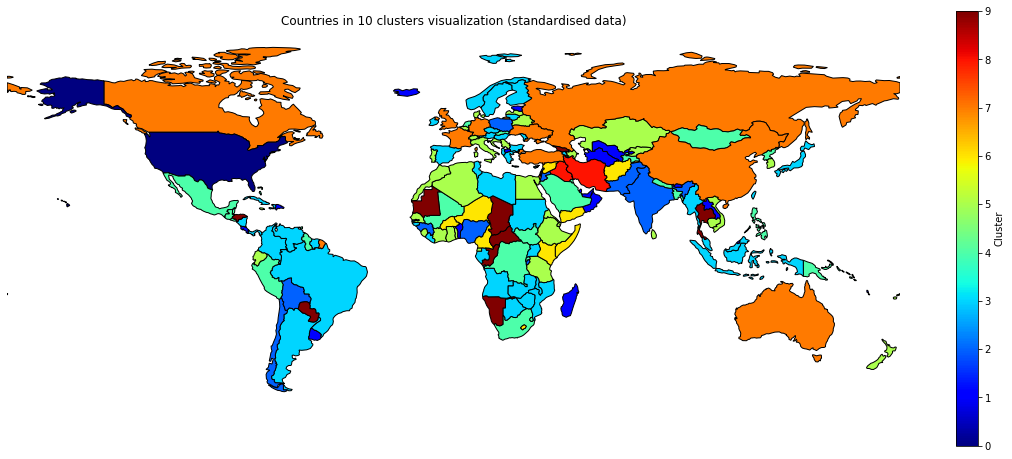
\includegraphics[width=1 \textwidth]{fig/CLUST/10clusterMap_std.png}
        \caption{Mapa z wynikami klasteryzacji. (źródło: opracowanie własne)}
        \label{fig:clust10std}
    \end{figure}

    Aby ułatwić interpretację wyników klasteryzacji poniżej dołączona została mapa~\ref{fig:clustPop} z naniesioną populacją oraz mapa~\ref{fig:clustGDP} z naniesionym PKB na osobę poszczególnych krajów, a także ich odpowiedniki ze skalą logarytmiczną~\ref{fig:clustPop_log} oraz~\ref{fig:clustGDP_log}.

    \begin{figure}[ht!]
        \centering
        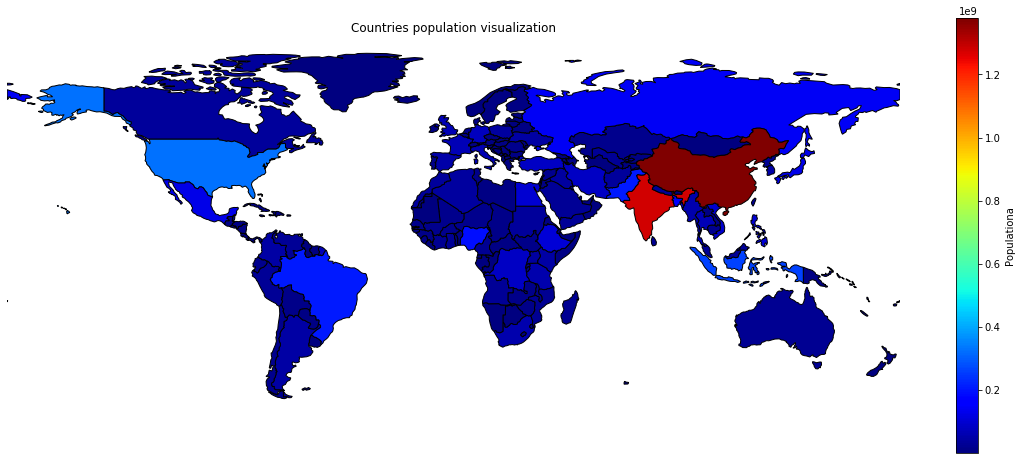
\includegraphics[width=1 \textwidth]{fig/CLUST/population.png}
        \caption{Mapa z populacją krajów. (źródło: opracowanie własne)}
        \label{fig:clustPop}
    \end{figure}

    \begin{figure}[ht!]
        \centering
        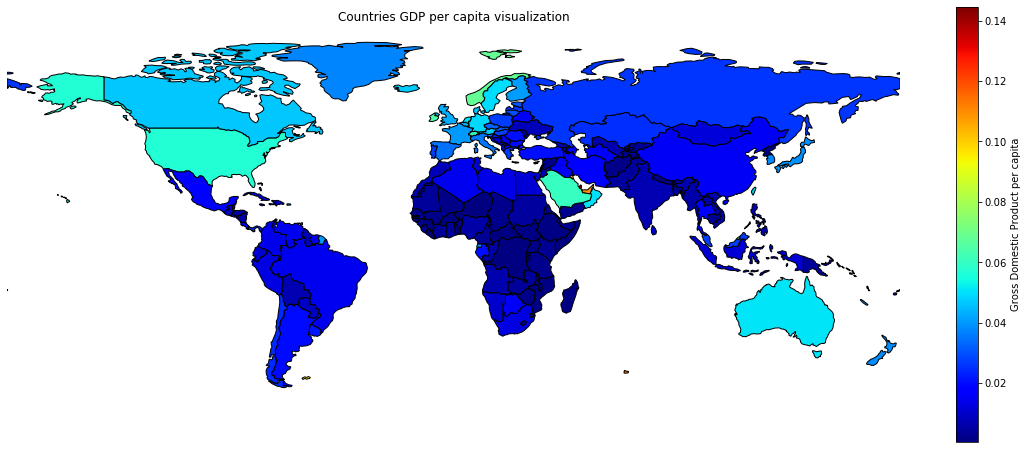
\includegraphics[width=1 \textwidth]{fig/CLUST/gdp.png}
        \caption{Mapa z PKP na osobę. (źródło: opracowanie własne)}
        \label{fig:clustGDP}
    \end{figure}

    \begin{figure}[ht!]
        \centering
        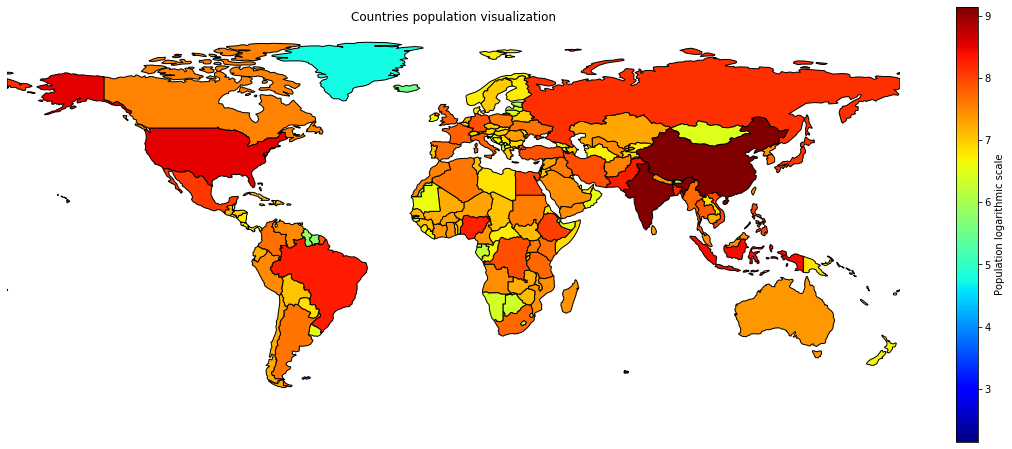
\includegraphics[width=1 \textwidth]{fig/CLUST/population_log.png}
        \caption{Mapa z populacją krajów - skala logarytmiczna. (źródło: opracowanie własne)}
        \label{fig:clustPop_log}
    \end{figure}

    \begin{figure}[ht!]
        \centering
        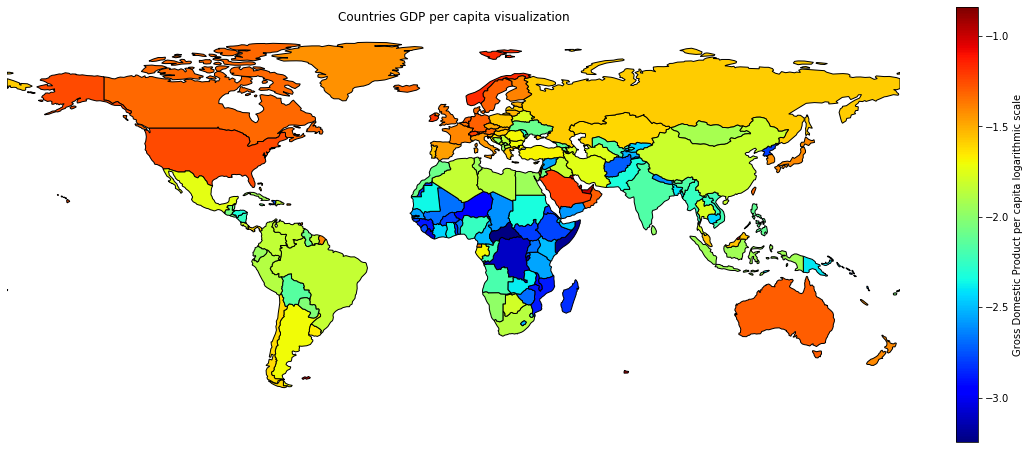
\includegraphics[width=1 \textwidth]{fig/CLUST/gdp_log.png}
        \caption{Mapa z PKB na osobę - skala logarytminczna. (źródło: opracowanie własne)}
        \label{fig:clustGDP_log}
    \end{figure}

    \begin{figure}[ht!]
        \centering
        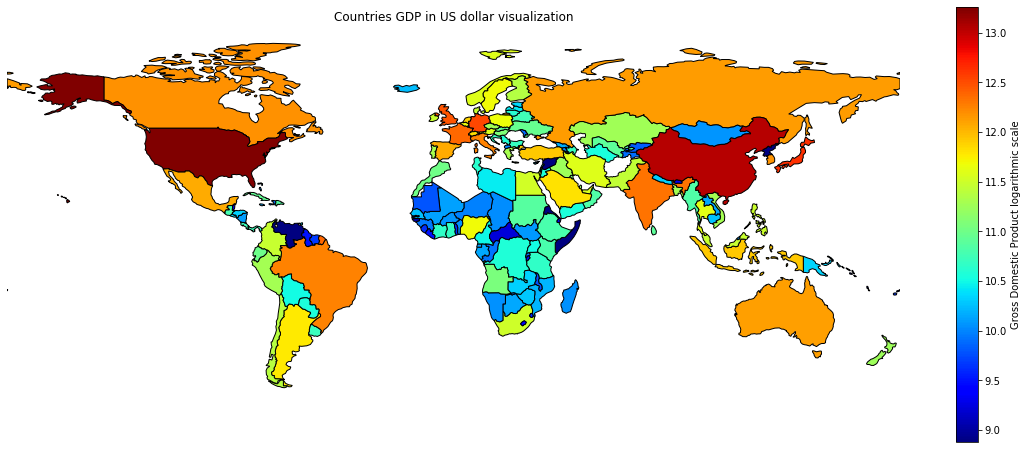
\includegraphics[width=1 \textwidth]{fig/CLUST/gdp2015.png}
        \caption{Mapa z PKB - skala logarytminczna. (źródło: opracowanie własne)}
        \label{fig:clustGDP2015_log}
    \end{figure}

    \begin{figure}[ht!]
        \centering
        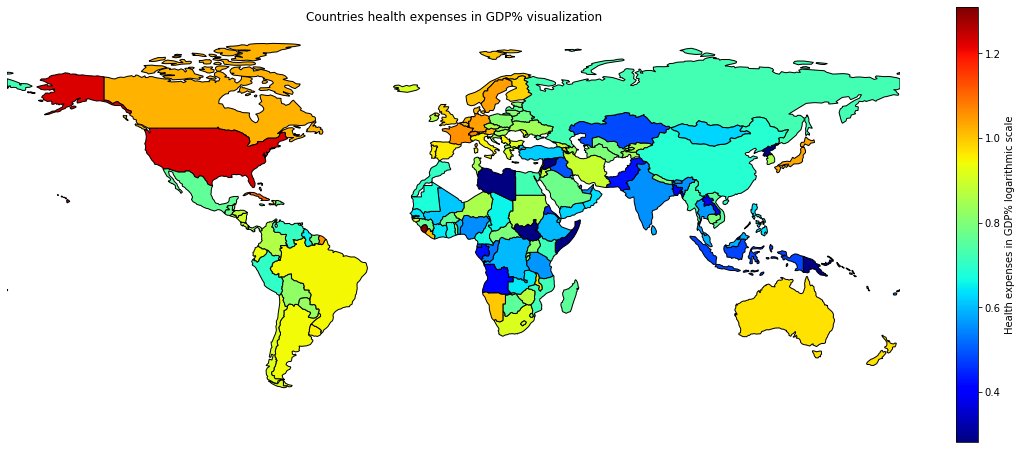
\includegraphics[width=1 \textwidth]{fig/CLUST/health2015.png}
        \caption{Mapa z wydatkami na zdrowie - skala logarytminczna. (źródło: opracowanie własne)}
        \label{fig:clustHealth2015_log}
    \end{figure}

    \begin{figure}[ht!]
        \centering
        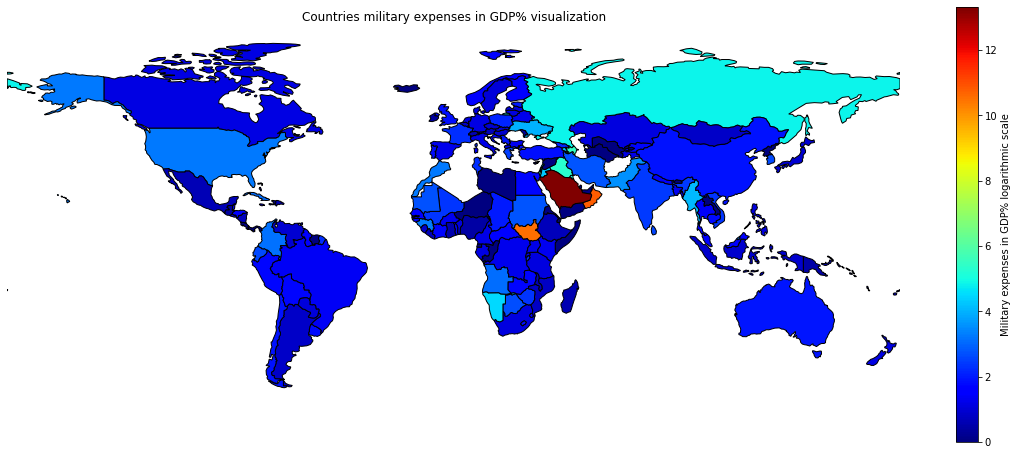
\includegraphics[width=1 \textwidth]{fig/CLUST/military2015.png}
        \caption{Mapa z wydatkami na zbrojenia - skala logarytminczna. (źródło: opracowanie własne)}
        \label{fig:clustMilitary2015_log}
    \end{figure}

    \begin{figure}[ht!]
        \centering
        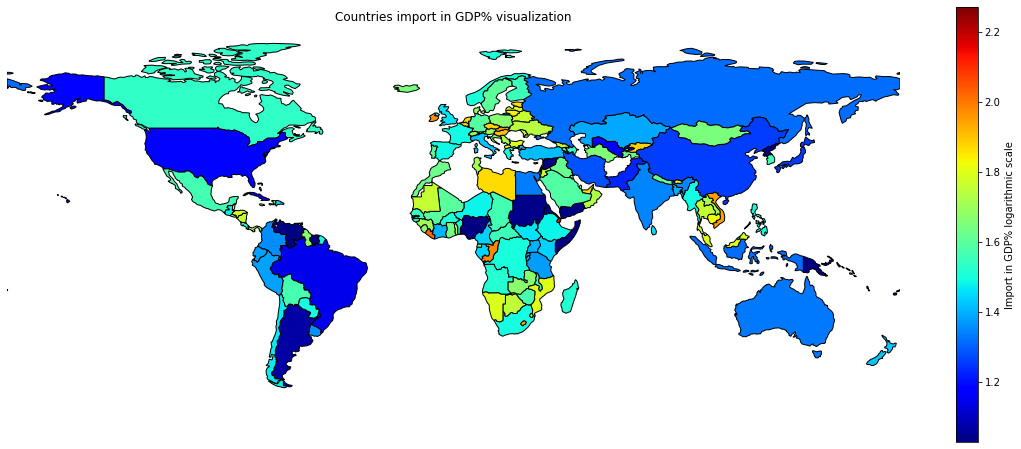
\includegraphics[width=1 \textwidth]{fig/CLUST/import2015.png}
        \caption{Mapa z importem - skala logarytminczna. (źródło: opracowanie własne)}
        \label{fig:clustImport2015_log}
    \end{figure}

    \begin{figure}[ht!]
        \centering
        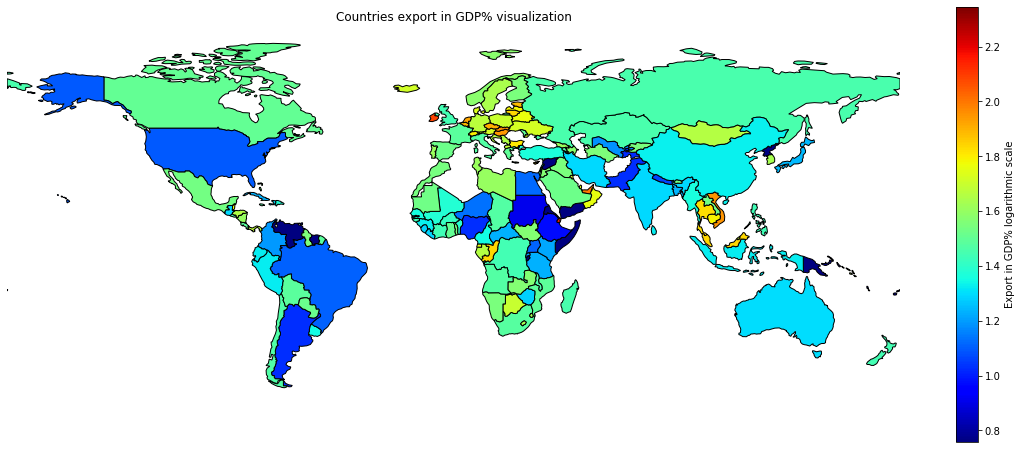
\includegraphics[width=1 \textwidth]{fig/CLUST/export2015.png}
        \caption{Mapa z eksportem - skala logarytminczna. (źródło: opracowanie własne)}
        \label{fig:clustExport2015_log}
    \end{figure}

%    todo: dodać opis pochodzenia danych

    \paragraph{Wyniki klasteryzacji w postacji tabelarycznej}
    W tabelach od~\ref{tab:cl0std} do~\ref{tab:cl9std} przedstawione zostały wyniki grupowania ustandaryzowanych próbek.
    Dodatkowo, jak przy danych niestandaryzowanych, zawarto informacje o liczbie ludności i PKB na osobę pochodzące z biblioteki GeoPandas~\cite{geopandas}.

    \begin{table}
    \centering
    \caption{Klaster 0 - dane standaryzowane}
    \label{tab:cl0std}
    \begin{tabular}{lrrrrrr}
        \toprule
        name                     & GDP     & health & military & education & imp & exp \\
        \midrule
        United States of America & 1.8e+13 & 17     & 3.3      & nan       & 15  & 12  \\
        \bottomrule
    \end{tabular}
\end{table}


    \begin{table}
    \centering
    \caption{Parametry klastra 0 - dane standaryzowane}
    \label{tab:cl0std_desc}
    \begin{tabular}{lrrrrr}
        \toprule
        {}                        & mean    & median  & std & min     & max     \\
        \midrule
        \textbf{avgGoldstein    }     & 0.37    & 0.37    & nan & 0.37    & 0.37    \\
        \textbf{imp             }              & 15      & 15      & nan & 15      & 15      \\
        \textbf{expressCount    }     & 2e+04   & 2e+04   & nan & 2e+04   & 2e+04   \\
        \textbf{sumNumMentions  }   & 3.5e+06 & 3.5e+06 & nan & 3.5e+06 & 3.5e+06 \\
        \textbf{materialConfCoop} & 0.16    & 0.16    & nan & 0.16    & 0.16    \\
        \textbf{fightCount      }       & 5.8e+04 & 5.8e+04 & nan & 5.8e+04 & 5.8e+04 \\
        \textbf{Events          }           & 8.2e+05 & 8.2e+05 & nan & 8.2e+05 & 8.2e+05 \\
        \textbf{verbalConfCoop  }   & 0.13    & 0.13    & nan & 0.13    & 0.13    \\
        \textbf{education       }        & nan     & nan     & nan & nan     & nan     \\
        \textbf{GDP             }              & 1.8e+13 & 1.8e+13 & nan & 1.8e+13 & 1.8e+13 \\
        \textbf{pop\_est         }         & 3.3e+08 & 3.3e+08 & nan & 3.3e+08 & 3.3e+08 \\
        \textbf{military        }         & 3.3     & 3.3     & nan & 3.3     & 3.3     \\
        \textbf{gdp\_per\_cap     }    & 0.057   & 0.057   & nan & 0.057   & 0.057   \\
        \textbf{exp             }              & 12      & 12      & nan & 12      & 12      \\
        \textbf{health          }           & 17      & 17      & nan & 17      & 17      \\
        \textbf{avgAvgTone      }       & -2.3    & -2.3    & nan & -2.3    & -2.3    \\
        \bottomrule
    \end{tabular}
\end{table}


    \begin{table}[h!]
    \centering
    \caption{Klaster 1 - dane standaryzowane}
    \label{tab:cl1std}
    \begin{tabular}{lllrr}
        \toprule
        iso\_a3 & name                 & continent     & pop\_est & gdp\_per\_cap \\
        \midrule
        BEN     & Benin                & Africa        & 11038805 & 0.002202      \\
        BTN     & Bhutan               & Asia          & 758288   & 0.008482      \\
        BRN     & Brunei               & Asia          & 443593   & 0.07604       \\
        CRI     & Costa Rica           & North America & 4930258  & 0.01608       \\
        DOM     & Dominican Rep.       & North America & 10734247 & 0.01508       \\
        EST     & Estonia              & Europe        & 1251581  & 0.03092       \\
        ISL     & Iceland              & Europe        & 339747   & 0.04754       \\
        LAO     & Laos                 & Asia          & 7126706  & 0.005747      \\
        LUX     & Luxembourg           & Europe        & 594130   & 0.09887       \\
        MKD     & Macedonia            & Europe        & 2103721  & 0.01403       \\
        MDG     & Madagascar           & Africa        & 25054161 & 0.001471      \\
        OMN     & Oman                 & Asia          & 3424386  & 0.05055       \\
        QAT     & Qatar                & Asia          & 2314307  & 0.1445        \\
        TKM     & Turkmenistan         & Asia          & 5351277  & 0.0177        \\
        ARE     & United Arab Emirates & Asia          & 6072475  & 0.1099        \\
        URY     & Uruguay              & South America & 3360148  & 0.0218        \\
        UZB     & Uzbekistan           & Asia          & 29748859 & 0.0068        \\
        VUT     & Vanuatu              & Oceania       & 282814   & 0.002556      \\
        \bottomrule
    \end{tabular}
\end{table}


    \begin{table}[h!]
    \centering
    \caption{Parametry klastra 1 - dane standaryzowane}
    \label{tab:cl1std_desc}
    \begin{tabular}{lrrrrr}
        \toprule
        {}                        & mean      & median    & std       & min       & max       \\
        \midrule
        \textbf{pop\_est         }         & 6.385e+06 & 3.392e+06 & 8.375e+06 & 2.828e+05 & 2.975e+07 \\
        \textbf{materialConfCoop} & 0.0653    & 0.06346   & 0.01573   & 0.0371    & 0.09901   \\
        \textbf{gdp\_per\_cap     }    & 0.03724   & 0.01689   & 0.04268   & 0.001471  & 0.1445    \\
        \textbf{fightCount      }       & 65.83     & 30.5      & 97.29     & 2.0       & 393.0     \\
        \textbf{verbalConfCoop  }   & 0.08207   & 0.07921   & 0.02208   & 0.04769   & 0.1257    \\
        \textbf{Events          }           & 2.421e+03 & 1.34e+03  & 2.923e+03 & 261.0     & 1.168e+04 \\
        \textbf{sumNumMentions  }   & 1.195e+04 & 7.182e+03 & 1.304e+04 & 1.42e+03  & 5.238e+04 \\
        \textbf{expressCount    }     & 32.83     & 22.5      & 37.63     & 1.0       & 160.0     \\
        \textbf{avgAvgTone      }       & -0.2539   & -0.2941   & 0.3794    & -0.9221   & 0.4018    \\
        \textbf{avgGoldstein    }     & 1.943     & 1.887     & 0.3279    & 1.476     & 2.749     \\
        \bottomrule
    \end{tabular}
\end{table}


    \begin{table}
    \centering
    \caption{Klaster 2 - dane standaryzowane}
    \label{tab:cl2std}
    \begin{tabular}{lrrrrrr}
        \toprule
        name      & GDP     & health & military & education & imp & exp \\
        \midrule
        Bolivia   & 3.3e+10 & 6.6    & 1.7      & nan       & 37  & 31  \\
        Burundi   & 3.1e+09 & 6.6    & 2.2      & 6.4       & 27  & 5.7 \\
        Chile     & 2.4e+11 & 8.3    & 1.9      & 4.9       & 30  & 29  \\
        Gambia    & 1.4e+09 & 3.1    & 1.5      & 2.1       & 33  & 16  \\
        Guinea    & 8.8e+09 & 5.8    & 3.3      & 2.5       & 51  & 21  \\
        India     & 2.1e+12 & 3.6    & 2.4      & nan       & 22  & 20  \\
        Jordan    & 3.8e+10 & 7.6    & 4.3      & nan       & 60  & 37  \\
        Lebanon   & 5e+10   & 7.7    & 4.5      & nan       & 49  & 23  \\
        Nigeria   & 4.9e+11 & 3.6    & 0.42     & nan       & 11  & 11  \\
        Pakistan  & 2.7e+11 & 2.7    & 3.6      & 2.7       & 17  & 11  \\
        Palestine & 1.3e+10 & nan    & nan      & 5.1       & 59  & 18  \\
        Poland    & 4.8e+11 & 6.4    & 2.1      & 4.8       & 46  & 49  \\
        \bottomrule
    \end{tabular}
\end{table}


    \begin{table}
    \centering
    \caption{Parametry klastra 2 - dane standaryzowane}
    \label{tab:cl2std_desc}
    \begin{tabular}{lrrrrr}
        \toprule
        {}                        & mean    & median  & std     & min     & max     \\
        \midrule
        \textbf{avgGoldstein    }     & 0.23    & 0.33    & 0.42    & -0.46   & 0.75    \\
        \textbf{imp             }              & 37      & 35      & 16      & 11      & 60      \\
        \textbf{expressCount    }     & 3.3e+02 & 2.1e+02 & 3.9e+02 & 13      & 1.4e+03 \\
        \textbf{sumNumMentions  }   & 8.6e+04 & 7.4e+04 & 7.1e+04 & 7.2e+03 & 2.3e+05 \\
        \textbf{materialConfCoop} & 0.14    & 0.13    & 0.029   & 0.092   & 0.19    \\
        \textbf{fightCount      }       & 1.1e+03 & 1e+03   & 1e+03   & 71      & 3e+03   \\
        \textbf{Events          }           & 1.9e+04 & 1.6e+04 & 1.7e+04 & 1.5e+03 & 5.2e+04 \\
        \textbf{verbalConfCoop  }   & 0.18    & 0.17    & 0.025   & 0.15    & 0.23    \\
        \textbf{education       }        & 4.1     & 4.8     & 1.6     & 2.1     & 6.4     \\
        \textbf{GDP             }              & 3.1e+11 & 4.4e+10 & 5.9e+11 & 1.4e+09 & 2.1e+12 \\
        \textbf{pop\_est         }         & 1.5e+08 & 1.2e+07 & 3.6e+08 & 2.1e+06 & 1.3e+09 \\
        \textbf{military        }         & 2.5     & 2.2     & 1.2     & 0.42    & 4.5     \\
        \textbf{gdp\_per\_cap     }    & 0.0089  & 0.0063  & 0.0087  & 0.00069 & 0.027   \\
        \textbf{exp             }              & 23      & 21      & 12      & 5.7     & 49      \\
        \textbf{health          }           & 5.6     & 6.4     & 2       & 2.7     & 8.3     \\
        \textbf{avgAvgTone      }       & -2.4    & -2.3    & 0.61    & -4.1    & -1.7    \\
        \bottomrule
    \end{tabular}
\end{table}


    \begin{table}
    \centering
    \caption{Klaster 3 - dane standaryzowane}
    \label{tab:cl3std}
    \begin{tabular}{lrrrrrr}
        \toprule
        name          & GDP     & health & military & education & imp     & exp     \\
        \midrule
        Angola        & 1.2e+11 & 2.6    & 3.1      & nan       & 33      & 30      \\
        Argentina     & 5.9e+11 & 8.8    & 0.85     & 5.8       & 12      & 11      \\
        Armenia       & 1.1e+10 & 10     & 4.2      & 2.8       & 42      & 30      \\
        Austria       & 3.8e+11 & 10     & 0.7      & 5.5       & 49      & 53      \\
        Botswana      & 1.4e+10 & 5.7    & 2.7      & nan       & 56      & 50      \\
        Brazil        & 1.8e+12 & 8.9    & 1.4      & 6.2       & 14      & 13      \\
        Bulgaria      & 5.1e+10 & 8.2    & 1.3      & nan       & 63      & 64      \\
        Colombia      & 2.9e+11 & 7.3    & 3.1      & 4.5       & 23      & 16      \\
        Cuba          & 8.7e+10 & 13     & 3.1      & nan       & 14      & 17      \\
        Cyprus        & 2e+10   & 6.8    & 1.7      & 6.4       & 68      & 70      \\
        Cyprus        & 2e+10   & 6.8    & 1.7      & 6.4       & 68      & 70      \\
        Czechia       & 1.9e+11 & 7.2    & 0.95     & 5.8       & 75      & 81      \\
        Finland       & 2.3e+11 & 9.7    & 1.5      & 7.1       & 36      & 35      \\
        Gabon         & 1.4e+10 & 2.7    & 1.2      & nan       & 28      & 46      \\
        Greece        & 2e+11   & 8.1    & 2.5      & nan       & 32      & 32      \\
        Guinea-Bissau & 1e+09   & 8.6    & 1.6      & nan       & 32      & 28      \\
        Haiti         & 8.7e+09 & 8.6    & 0.00089  & 3.2       & 51      & 20      \\
        Hungary       & 1.2e+11 & 7      & 0.92     & 4.6       & 80      & 88      \\
        Indonesia     & 8.6e+11 & 3      & 0.89     & 3.6       & 21      & 21      \\
        Ireland       & 2.9e+11 & 7.3    & 0.34     & 3.8       & 93      & 1.2e+02 \\
        Japan         & 4.4e+12 & 11     & 0.96     & nan       & 18      & 18      \\
        Liberia       & 3.2e+09 & 10     & 0.73     & nan       & 1.1e+02 & 19      \\
        Libya         & 2.8e+10 & nan    & nan      & nan       & 74      & 40      \\
        Lithuania     & 4.1e+10 & 6.5    & 1.1      & 4.2       & 70      & 69      \\
        Malawi        & 6.4e+09 & 9.3    & 0.63     & 5.6       & 36      & 29      \\
        Malaysia      & 3e+11   & 3.9    & 1.5      & 5         & 62      & 69      \\
        Moldova       & 7.7e+09 & 8.6    & 0.35     & nan       & 57      & 32      \\
        Mozambique    & 1.6e+10 & 5.3    & 0.81     & nan       & 63      & 31      \\
        Myanmar       & 6.8e+10 & 5.2    & 4.1      & nan       & 31      & 23      \\
        N. Cyprus     & 2e+10   & 6.8    & 1.7      & 6.4       & 68      & 70      \\
        N. Cyprus     & 2e+10   & 6.8    & 1.7      & 6.4       & 68      & 70      \\
        Nicaragua     & 1.3e+10 & 8      & 0.78     & 4.1       & 58      & 40      \\
        Norway        & 3.9e+11 & 10     & 1.5      & 7.6       & 32      & 38      \\
        Panama        & 5.4e+10 & 6.8    & 0        & nan       & 52      & 48      \\
        Spain         & 1.2e+12 & 9.1    & 1.3      & 4.3       & 31      & 34      \\
        Sudan         & 7.4e+10 & 7.2    & 2.8      & nan       & 11      & 8.2     \\
        Suriname      & 4.8e+09 & 6.2    & nan      & nan       & nan     & nan     \\
        Sweden        & 5.1e+11 & 11     & 1.1      & 7.5       & 40      & 44      \\
        Tunisia       & 4.3e+10 & 7      & 2.3      & 6.6       & 52      & 41      \\
        Uganda        & 3.2e+10 & 6.5    & 1.2      & 2.8       & 25      & 13      \\
        Venezuela     & nan     & 5.1    & 0.94     & nan       & nan     & nan     \\
        Zambia        & 2.1e+10 & 4.4    & 1.8      & 4.6       & 47      & 37      \\
        Zimbabwe      & 2e+10   & 7.5    & 2.3      & nan       & 38      & 19      \\
        \bottomrule
    \end{tabular}
\end{table}


    \begin{table}
    \centering
    \caption{Parametry klastra 3 - dane standaryzowane}
    \label{tab:cl3std_desc}
    \begin{tabular}{lrrrrr}
        \toprule
        {}                        & mean    & median  & std     & min     & max     \\
        \midrule
        \textbf{avgGoldstein    }     & 0.97    & 0.97    & 0.25    & 0.49    & 1.4     \\
        \textbf{imp             }              & 47      & 47      & 23      & 11      & 1.1e+02 \\
        \textbf{expressCount    }     & 1.9e+02 & 1.1e+02 & 2.2e+02 & 3       & 9.3e+02 \\
        \textbf{sumNumMentions  }   & 4.8e+04 & 3.4e+04 & 5e+04   & 9.4e+02 & 2e+05   \\
        \textbf{materialConfCoop} & 0.11    & 0.12    & 0.021   & 0.011   & 0.13    \\
        \textbf{fightCount      }       & 3.9e+02 & 2.4e+02 & 5e+02   & 0       & 2.7e+03 \\
        \textbf{Events          }           & 9.1e+03 & 5.9e+03 & 9.5e+03 & 2.8e+02 & 3.9e+04 \\
        \textbf{verbalConfCoop  }   & 0.13    & 0.13    & 0.016   & 0.1     & 0.19    \\
        \textbf{education       }        & 5.2     & 5.5     & 1.4     & 2.8     & 7.6     \\
        \textbf{GDP             }              & 3e+11   & 4.7e+10 & 7.4e+11 & 1e+09   & 4.4e+12 \\
        \textbf{pop\_est         }         & 2.7e+07 & 1e+07   & 5.2e+07 & 2.7e+05 & 2.6e+08 \\
        \textbf{military        }         & 1.5     & 1.3     & 1       & 0       & 4.2     \\
        \textbf{gdp\_per\_cap     }    & 0.019   & 0.014   & 0.017   & 0.00083 & 0.069   \\
        \textbf{exp             }              & 41      & 35      & 25      & 8.2     & 1.2e+02 \\
        \textbf{health          }           & 7.5     & 7.3     & 2.3     & 2.6     & 13      \\
        \textbf{avgAvgTone      }       & -1.6    & -1.7    & 0.5     & -2.5    & -0.23   \\
        \bottomrule
    \end{tabular}
\end{table}


    \begin{table}[h!]
    \centering
    \caption{Klaster 4 - dane standaryzowane}
    \label{tab:cl4std}
    \begin{tabular}{lllrr}
        \toprule
        iso\_a3 & name                & continent     & pop\_est  & gdp\_per\_cap \\
        \midrule
        BHS     & Bahamas             & North America & 329988    & 0.02747       \\
        BGD     & Bangladesh          & Asia          & 157826578 & 0.003982      \\
        BLZ     & Belize              & North America & 360346    & 0.00857       \\
        COD     & Dem. Rep. Congo     & Africa        & 83301151  & 0.0007924     \\
        SLV     & El Salvador         & North America & 6172011   & 0.008877      \\
        GTM     & Guatemala           & North America & 15460732  & 0.008525      \\
        GUY     & Guyana              & South America & 737718    & 0.008259      \\
        KWT     & Kuwait              & Asia          & 2875422   & 0.1047        \\
        MLI     & Mali                & Africa        & 17885245  & 0.00213       \\
        MEX     & Mexico              & North America & 124574795 & 0.01852       \\
        MNG     & Mongolia            & Asia          & 3068243   & 0.01206       \\
        NPL     & Nepal               & Asia          & 29384297  & 0.002434      \\
        NLD     & Netherlands         & Europe        & 17084719  & 0.05097       \\
        PRK     & North Korea         & Asia          & 25248140  & 0.001584      \\
        PNG     & Papua New Guinea    & Oceania       & 6909701   & 0.004055      \\
        PER     & Peru                & South America & 31036656  & 0.01322       \\
        PHL     & Philippines         & Asia          & 104256076 & 0.007692      \\
        RWA     & Rwanda              & Africa        & 11901484  & 0.001846      \\
        SSD     & S. Sudan            & Africa        & 13026129  & 0.001603      \\
        SAU     & Saudi Arabia        & Asia          & 28571770  & 0.06058       \\
        SVK     & Slovakia            & Europe        & 5445829   & 0.031         \\
        SLB     & Solomon Is.         & Oceania       & 647581    & 0.00185       \\
        ZAF     & South Africa        & Africa        & 54841552  & 0.01348       \\
        TJK     & Tajikistan          & Asia          & 8468555   & 0.003048      \\
        TTO     & Trinidad and Tobago & North America & 1218208   & 0.03577       \\
        SWZ     & eSwatini            & Africa        & 1467152   & 0.007538      \\
        \bottomrule
    \end{tabular}
\end{table}


    \begin{table}[h!]
    \centering
    \caption{Parametry klastra 4 - dane standaryzowane}
    \label{tab:cl4std_desc}
    \begin{tabular}{lrrrrr}
        \toprule
        {}                        & mean      & median    & std       & min       & max       \\
        \midrule
        \textbf{pop\_est         }         & 2.893e+07 & 1.246e+07 & 4.202e+07 & 3.3e+05   & 1.578e+08 \\
        \textbf{materialConfCoop} & 0.1634    & 0.1614    & 0.02405   & 0.1272    & 0.2331    \\
        \textbf{gdp\_per\_cap     }    & 0.01694   & 0.008392  & 0.02373   & 0.0007924 & 0.1047    \\
        \textbf{fightCount      }       & 424.1     & 173.0     & 629.0     & 5.0       & 2.417e+03 \\
        \textbf{verbalConfCoop  }   & 0.1035    & 0.1078    & 0.02079   & 0.04282   & 0.1311    \\
        \textbf{Events          }           & 6.648e+03 & 2.708e+03 & 8.592e+03 & 206.0     & 3.564e+04 \\
        \textbf{sumNumMentions  }   & 3.249e+04 & 1.279e+04 & 4.267e+04 & 895.0     & 1.926e+05 \\
        \textbf{expressCount    }     & 145.7     & 62.5      & 196.8     & 4.0       & 749.0     \\
        \textbf{avgAvgTone      }       & -2.082    & -2.021    & 0.6532    & -3.673    & -1.062    \\
        \textbf{avgGoldstein    }     & 0.5751    & 0.5574    & 0.2709    & -0.0144   & 1.054     \\
        \bottomrule
    \end{tabular}
\end{table}


    \begin{table}
    \centering
    \caption{Klaster 5 - dane standaryzowane}
    \label{tab:cl5std}
    \begin{tabular}{lrrrrrr}
        \toprule
        name          & GDP     & health & military & education & imp     & exp     \\
        \midrule
        Azerbaijan    & 5.3e+10 & 6.7    & 5.5      & 3         & 35      & 38      \\
        Belarus       & 5.6e+10 & 6.1    & 1.3      & 4.8       & 58      & 58      \\
        Belgium       & 4.6e+11 & 10     & 0.92     & 6.5       & 76      & 78      \\
        Cambodia      & 1.8e+10 & 6.2    & 1.8      & nan       & 66      & 62      \\
        Croatia       & 5e+10   & 6.8    & 1.5      & nan       & 46      & 46      \\
        Côte d'Ivoire & 4.6e+10 & 4.4    & 1.7      & 4.8       & 25      & 27      \\
        Denmark       & 3e+11   & 10     & 1.1      & nan       & 49      & 55      \\
        Djibouti      & 2.4e+09 & 4.4    & nan      & 5.3       & 1.2e+02 & 1.4e+02 \\
        Ecuador       & 9.9e+10 & 8.6    & 2.6      & 5         & 24      & 21      \\
        Egypt         & 3.3e+11 & 5.3    & 1.7      & nan       & 22      & 13      \\
        Eq. Guinea    & 1.3e+10 & 2.9    & nan      & nan       & 42      & 57      \\
        Eritrea       & nan     & 2.9    & nan      & nan       & nan     & nan     \\
        Ethiopia      & 6.5e+10 & 3.9    & 0.71     & 4.7       & 30      & 9.4     \\
        Fiji          & 4.7e+09 & 3.6    & 0.97     & nan       & nan     & nan     \\
        Ghana         & 4.9e+10 & 4.6    & 0.53     & 4.5       & 44      & 32      \\
        Italy         & 1.8e+12 & 9      & 1.2      & 4.1       & 27      & 30      \\
        Jamaica       & 1.4e+10 & 5.7    & 0.87     & 5.5       & 46      & 30      \\
        Kazakhstan    & 1.8e+11 & 3      & 1.1      & 2.8       & 25      & 29      \\
        Kyrgyzstan    & 6.7e+09 & 7.1    & 1.8      & 6         & 76      & 35      \\
        Latvia        & 2.7e+10 & 5.7    & 1        & 5.3       & 62      & 61      \\
        Morocco       & 1e+11   & 5.1    & 3.2      & nan       & 42      & 35      \\
        New Zealand   & 1.8e+11 & 9.3    & 1.1      & 6.3       & 27      & 28      \\
        Portugal      & 2e+11   & 9      & 1.8      & 4.9       & 40      & 41      \\
        Senegal       & 1.8e+10 & 4.4    & 1.6      & 5.5       & 35      & 23      \\
        Serbia        & 4e+10   & 8.8    & 1.9      & 3.8       & 52      & 45      \\
        Sierra Leone  & 4.2e+09 & 20     & 0.92     & nan       & 47      & 19      \\
        South Korea   & 1.5e+12 & 7      & 2.6      & nan       & 36      & 43      \\
        Sri Lanka     & 8.1e+10 & 3.9    & 2.6      & 2.2       & 29      & 21      \\
        Switzerland   & 6.8e+11 & 12     & 0.67     & 5.1       & 51      & 62      \\
        Tanzania      & 4.7e+10 & 3.6    & 1.1      & nan       & 24      & 17      \\
        Togo          & 4.2e+09 & 6.2    & 1.7      & 5.1       & 58      & 36      \\
        Vietnam       & 1.9e+11 & 5.7    & 2.4      & nan       & 89      & 90      \\
        \bottomrule
    \end{tabular}
\end{table}


    \begin{table}[h!]
    \centering
    \caption{Parametry klastra 5 - dane standaryzowane}
    \label{tab:cl5std_desc}
    \begin{tabular}{lrrrrr}
        \toprule
        {}                        & mean      & median    & std       & min       & max       \\
        \midrule
        \textbf{pop\_est         }         & 2.38e+07  & 1.084e+07 & 2.907e+07 & 7.784e+05 & 1.054e+08 \\
        \textbf{materialConfCoop} & 0.09779   & 0.1005    & 0.01777   & 0.06512   & 0.1308    \\
        \textbf{gdp\_per\_cap     }    & 0.01711   & 0.0112    & 0.0161    & 0.001458  & 0.06026   \\
        \textbf{fightCount      }       & 267.9     & 143.0     & 312.8     & 9.0       & 1.529e+03 \\
        \textbf{verbalConfCoop  }   & 0.09955   & 0.1004    & 0.01481   & 0.06468   & 0.1241    \\
        \textbf{Events          }           & 7.575e+03 & 5.457e+03 & 8.408e+03 & 407.0     & 3.717e+04 \\
        \textbf{sumNumMentions  }   & 3.961e+04 & 3.063e+04 & 4.565e+04 & 1.952e+03 & 2.152e+05 \\
        \textbf{expressCount    }     & 148.4     & 69.0      & 189.7     & 2.0       & 877.0     \\
        \textbf{avgAvgTone      }       & -0.9773   & -1.015    & 0.4199    & -1.774    & -0.2663   \\
        \textbf{avgGoldstein    }     & 1.394     & 1.405     & 0.2514    & 0.9687    & 2.107     \\
        \bottomrule
    \end{tabular}
\end{table}


    \begin{table}[h!]
    \centering
    \caption{Klaster 6 - dane standaryzowane}
    \label{tab:cl6std}
    \begin{tabular}{lllrr}
        \toprule
        iso\_a3 & name         & continent & pop\_est & gdp\_per\_cap \\
        \midrule
        AFG     & Afghanistan  & Asia      & 34124811 & 0.001878      \\
        BFA     & Burkina Faso & Africa    & 20107509 & 0.001641      \\
        CMR     & Cameroon     & Africa    & 24994885 & 0.00309       \\
        KEN     & Kenya        & Africa    & 47615739 & 0.003207      \\
        LSO     & Lesotho      & Africa    & 1958042  & 0.003074      \\
        NER     & Niger        & Africa    & 19245344 & 0.001047      \\
        SOM     & Somalia      & Africa    & 7531386  & 0.0006266     \\
        SYR     & Syria        & Asia      & 18028549 & 0.002789      \\
        YEM     & Yemen        & Asia      & 28036829 & 0.00262       \\
        \bottomrule
    \end{tabular}
\end{table}


    \begin{table}[h!]
    \centering
    \caption{Parametry klastra 6 - dane standaryzowane}
    \label{tab:cl6std_desc}
    \begin{tabular}{lrrrrr}
        \toprule
        {}                        & mean      & median    & std       & min       & max       \\
        \midrule
        \textbf{pop\_est         }         & 2.24e+07  & 2.011e+07 & 1.362e+07 & 1.958e+06 & 4.762e+07 \\
        \textbf{materialConfCoop} & 0.2495    & 0.2284    & 0.04484   & 0.1877    & 0.3138    \\
        \textbf{gdp\_per\_cap     }    & 0.002219  & 0.00262   & 0.000956  & 0.0006266 & 0.003207  \\
        \textbf{fightCount      }       & 1.576e+03 & 1.031e+03 & 1.79e+03  & 157.0     & 5.644e+03 \\
        \textbf{verbalConfCoop  }   & 0.1111    & 0.112     & 0.02074   & 0.08095   & 0.1438    \\
        \textbf{Events          }           & 8.799e+03 & 5.091e+03 & 9.324e+03 & 1.071e+03 & 2.747e+04 \\
        \textbf{sumNumMentions  }   & 4.079e+04 & 2.249e+04 & 4.22e+04  & 5.154e+03 & 1.235e+05 \\
        \textbf{expressCount    }     & 120.1     & 46.0      & 141.5     & 12.0      & 425.0     \\
        \textbf{avgAvgTone      }       & -3.785    & -3.754    & 0.6074    & -4.501    & -2.797    \\
        \textbf{avgGoldstein    }     & -0.7943   & -0.5985   & 0.4934    & -1.679    & -0.2817   \\
        \bottomrule
    \end{tabular}
\end{table}


    \begin{table}
    \centering
    \caption{Klaster 7 - dane standaryzowane}
    \label{tab:cl7std}
    \begin{tabular}{lrrrrrr}
        \toprule
        name           & GDP     & health & military & education & imp & exp \\
        \midrule
        Australia      & 1.4e+12 & 9.3    & 2        & 5.3       & 22  & 20  \\
        Canada         & 1.6e+12 & 11     & 1.2      & nan       & 34  & 32  \\
        China          & 1.1e+13 & 4.9    & 1.9      & nan       & 18  & 21  \\
        France         & 2.4e+12 & 11     & 2.3      & nan       & 31  & 31  \\
        Germany        & 3.4e+12 & 11     & 1.2      & 4.8       & 39  & 47  \\
        Israel         & 3e+11   & 7.1    & 5.6      & 5.9       & 28  & 31  \\
        Russia         & 1.4e+12 & 5.3    & 4.9      & 3.8       & 21  & 29  \\
        Turkey         & 8.6e+11 & 4.1    & 1.8      & nan       & 26  & 23  \\
        Ukraine        & 9.1e+10 & 6.9    & 4        & nan       & 55  & 53  \\
        United Kingdom & 2.9e+12 & 9.7    & 1.9      & 5.6       & 29  & 28  \\
        \bottomrule
    \end{tabular}
\end{table}


    \begin{table}
    \centering
    \caption{Parametry klastra 7 - dane standaryzowane}
    \label{tab:cl7std_desc}
    \begin{tabular}{lrrrrr}
        \toprule
        {}                        & mean    & median  & std     & min     & max     \\
        \midrule
        \textbf{avgGoldstein    }     & 0.84    & 0.96    & 0.45    & 0.011   & 1.4     \\
        \textbf{imp             }              & 30      & 29      & 11      & 18      & 55      \\
        \textbf{expressCount    }     & 2e+03   & 1.9e+03 & 8.2e+02 & 9.1e+02 & 3.2e+03 \\
        \textbf{sumNumMentions  }   & 4.4e+05 & 3.7e+05 & 1.6e+05 & 3e+05   & 7.5e+05 \\
        \textbf{materialConfCoop} & 0.13    & 0.12    & 0.023   & 0.099   & 0.16    \\
        \textbf{fightCount      }       & 5e+03   & 5e+03   & 1.7e+03 & 2.8e+03 & 7.6e+03 \\
        \textbf{Events          }           & 9.2e+04 & 7.5e+04 & 3.4e+04 & 6.3e+04 & 1.6e+05 \\
        \textbf{verbalConfCoop  }   & 0.12    & 0.12    & 0.015   & 0.1     & 0.14    \\
        \textbf{education       }        & 5.1     & 5.3     & 0.8     & 3.8     & 5.9     \\
        \textbf{GDP             }              & 2.5e+12 & 1.5e+12 & 3.2e+12 & 9.1e+10 & 1.1e+13 \\
        \textbf{pop\_est         }         & 1.9e+08 & 6.6e+07 & 4.2e+08 & 8.3e+06 & 1.4e+09 \\
        \textbf{military        }         & 2.7     & 1.9     & 1.6     & 1.2     & 5.6     \\
        \textbf{gdp\_per\_cap     }    & 0.034   & 0.038   & 0.015   & 0.008   & 0.051   \\
        \textbf{exp             }              & 31      & 30      & 11      & 20      & 53      \\
        \textbf{health          }           & 8       & 8.2     & 2.7     & 4.1     & 11      \\
        \textbf{avgAvgTone      }       & -2.2    & -2.2    & 0.47    & -3.2    & -1.4    \\
        \bottomrule
    \end{tabular}
\end{table}


    \begin{table}
    \centering
    \caption{Klaster 8 - dane standaryzowane}
    \label{tab:cl8std}
    \begin{tabular}{lrrrrrr}
        \toprule
        name & GDP     & health & military & education & imp & exp \\
        \midrule
        Iran & 3.8e+11 & 7.8    & 2.8      & 2.8       & 19  & 20  \\
        Iraq & 1.8e+11 & 3.1    & 5.3      & nan       & 41  & 35  \\
        \bottomrule
    \end{tabular}
\end{table}


    \begin{table}[h!]
    \centering
    \caption{Parametry klastra 8 - dane standaryzowane}
    \label{tab:cl8std_desc}
    \begin{tabular}{lrrrrr}
        \toprule
        {}                        & mean      & median    & std       & min       & max       \\
        \midrule
        \textbf{pop\_est         }         & 6.061e+07 & 6.061e+07 & 3.028e+07 & 3.919e+07 & 8.202e+07 \\
        \textbf{materialConfCoop} & 0.2898    & 0.2898    & 0.01858   & 0.2766    & 0.3029    \\
        \textbf{gdp\_per\_cap     }    & 0.01651   & 0.01651   & 0.001812  & 0.01523   & 0.01779   \\
        \textbf{fightCount      }       & 2.398e+04 & 2.398e+04 & 1.295e+04 & 1.483e+04 & 3.314e+04 \\
        \textbf{verbalConfCoop  }   & 0.1825    & 0.1825    & 0.02016   & 0.1683    & 0.1968    \\
        \textbf{Events          }           & 1.216e+05 & 1.216e+05 & 6.94e+04  & 7.254e+04 & 1.707e+05 \\
        \textbf{sumNumMentions  }   & 5.195e+05 & 5.195e+05 & 2.915e+05 & 3.134e+05 & 7.256e+05 \\
        \textbf{expressCount    }     & 1.372e+03 & 1.372e+03 & 1.224e+03 & 507.0     & 2.238e+03 \\
        \textbf{avgAvgTone      }       & -4.501    & -4.501    & 0.01991   & -4.515    & -4.487    \\
        \textbf{avgGoldstein    }     & -1.837    & -1.837    & 0.06262   & -1.881    & -1.793    \\
        \bottomrule
    \end{tabular}
\end{table}


    \begin{table}
    \centering
    \caption{Klaster 9 - dane standaryzowane}
    \label{tab:cl9std}
    \begin{tabular}{lrrrrrr}
        \toprule
        name                 & GDP     & health & military & education & imp & exp \\
        \midrule
        Central African Rep. & 1.7e+09 & 6.3    & 1.7      & nan       & 36  & 17  \\
        Chad                 & 1.1e+10 & 4.5    & 2        & nan       & 37  & 30  \\
        Congo                & 8.6e+09 & 3.4    & nan      & 4.6       & 96  & 69  \\
        Georgia              & 1.5e+10 & 7.9    & 2.1      & nan       & 58  & 41  \\
        Honduras             & 2.1e+10 & 7.7    & 1.7      & 6.4       & 62  & 45  \\
        Mauritania           & 6.2e+09 & 4.7    & 2.8      & nan       & 57  & 34  \\
        Namibia              & 1.1e+10 & 9.9    & 4.5      & nan       & 62  & 36  \\
        Paraguay             & 3.6e+10 & 6.7    & 1.1      & nan       & 32  & 33  \\
        Thailand             & 4e+11   & 3.7    & 1.4      & nan       & 57  & 68  \\
        \bottomrule
    \end{tabular}
\end{table}


    \begin{table}
    \centering
    \caption{Parametry klastra 9 - dane standaryzowane}
    \label{tab:cl9std_desc}
    \begin{tabular}{lrrrrr}
        \toprule
        {}                        & mean    & median  & std     & min     & max     \\
        \midrule
        \textbf{avgGoldstein    }     & 1       & 1.1     & 0.4     & 0.45    & 1.7     \\
        \textbf{imp             }              & 55      & 57      & 20      & 32      & 96      \\
        \textbf{expressCount    }     & 65      & 37      & 99      & 0       & 3.1e+02 \\
        \textbf{sumNumMentions  }   & 1.2e+04 & 6.3e+03 & 1.3e+04 & 66      & 4.2e+04 \\
        \textbf{materialConfCoop} & 0.12    & 0.13    & 0.053   & 0       & 0.18    \\
        \textbf{fightCount      }       & 1.3e+02 & 84      & 1.2e+02 & 0       & 3.5e+02 \\
        \textbf{Events          }           & 2.4e+03 & 1.3e+03 & 2.6e+03 & 20      & 8.4e+03 \\
        \textbf{verbalConfCoop  }   & 0.07    & 0.079   & 0.027   & 0       & 0.09    \\
        \textbf{education       }        & 5.5     & 5.5     & 1.3     & 4.6     & 6.4     \\
        \textbf{GDP             }              & 5.7e+10 & 1.1e+10 & 1.3e+11 & 1.7e+09 & 4e+11   \\
        \textbf{pop\_est         }         & 1.3e+07 & 5.6e+06 & 2.1e+07 & 2.5e+06 & 6.8e+07 \\
        \textbf{military        }         & 2.2     & 1.9     & 1.1     & 1.1     & 4.5     \\
        \textbf{gdp\_per\_cap     }    & 0.007   & 0.0061  & 0.0049  & 0.00057 & 0.017   \\
        \textbf{exp             }              & 41      & 36      & 17      & 17      & 69      \\
        \textbf{health          }           & 6.1     & 6.3     & 2.2     & 3.4     & 9.9     \\
        \textbf{avgAvgTone      }       & -2.9    & -2.8    & 0.57    & -3.9    & -2      \\
        \bottomrule
    \end{tabular}
\end{table}



    Zarówno dla danych nie poddanych oraz poddanych standaryzacji Stany Zjednoczono otrzymały własny klaster -~\ref{tab:cl7} oraz ~\ref{tab:cl0std}.
    Jest to spowodowane znaczącą przewagą liczby zdarzeń w porównaniu z innymi krajami.

    Dla danych standaryzowanych Polska jest jedynym krajem europejskim w klastrze~\ref{tab:cl2std}.
    Irak oraz Iran otrzymały własny klaster~\ref{tab:cl8std}.
    Wyróżnia się mniejsza grupa~\ref{tab:cl7std} w której znalazły się między innymi: Chiny, Francja, Niemcy, Rosja, Wielka Brytania.


    \chapter{Podsumowanie}
    W niniejszej części zostaną opisane wnioski z pracy według kolejności wcześniej przedstawionych rozdziałów.


    \section{Dalsze kierunki rozwoju}
    W tej części zostaną opisane możliwe kierunki rozwoju pracy.

    \paragraph{Analiza pod kątem COVID-19}

    \paragraph{Analiza pod kątem grup etnicznych}

    \paragraph{Analiza pod kątem grup religijnych}


    \inputencoding{utf8}

    \newpage
    \addcontentsline{toc}{chapter}{Bibliografia}
    \printbibliography[title={Bibliografia}]

\end{document}
